% !TeX spellcheck = en_US
\chapter{Application on Simulated Data}

The parameterization strategy introduced in chapter~\ref{chap:param_strategy} can now be applied to the simulation results from \geant. In the following sections, some comparisons and results are shown and discussed.

\section{Wavelength Binning}\label{sec:wvl_binning}

Since the photon detection efficiency of the SiPMs is a non-constant function of the wavelength (cf. figure~\ref{sipm:pde}), one can optimize the different wavelength ranges or \textit{bin sizes}~$\Delta\lambda$ by equalizing not the bin sizes (\textit{constant binning}) but the detected photons per bin which is further referred to as \textit{adaptive binning}. Figure~\ref{param:wvl_binning} shows a comparison between constant and adaptive wavelength binning.

\begin{figure}[H]
	\centering
	\begin{subfigure}[t]{0.49\textwidth}
		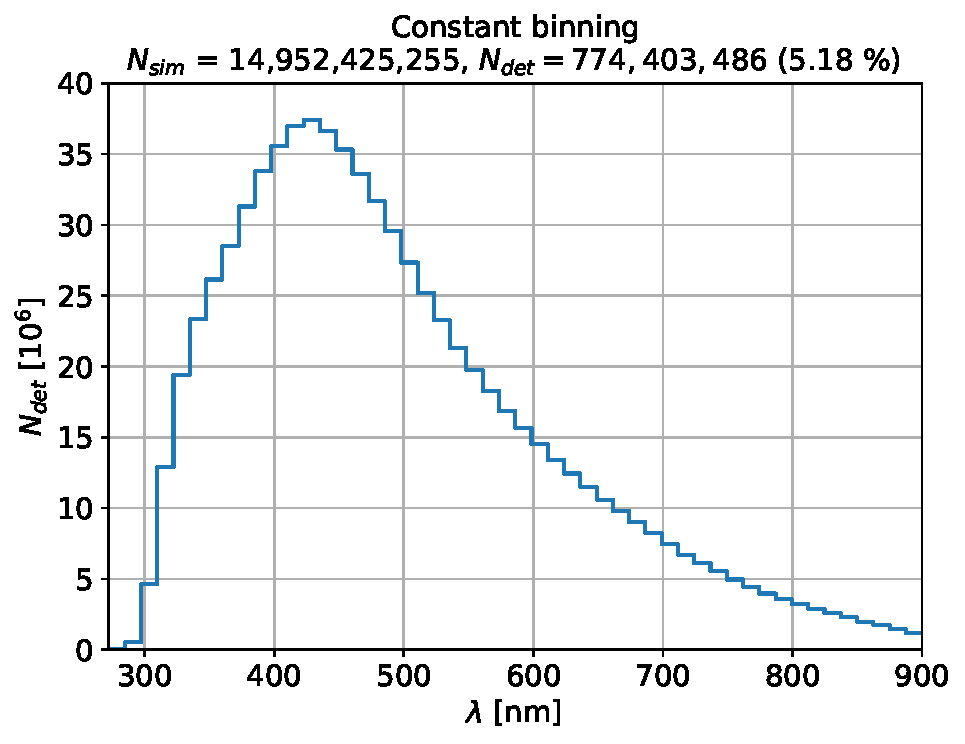
\includegraphics[width=\textwidth]{constant_wvl_bins_hist.pdf}
		\subcaption{constant binning}
		\label{param:wvl_binning:constant}
	\end{subfigure}
	\hfill
	\begin{subfigure}[t]{0.49\textwidth}
		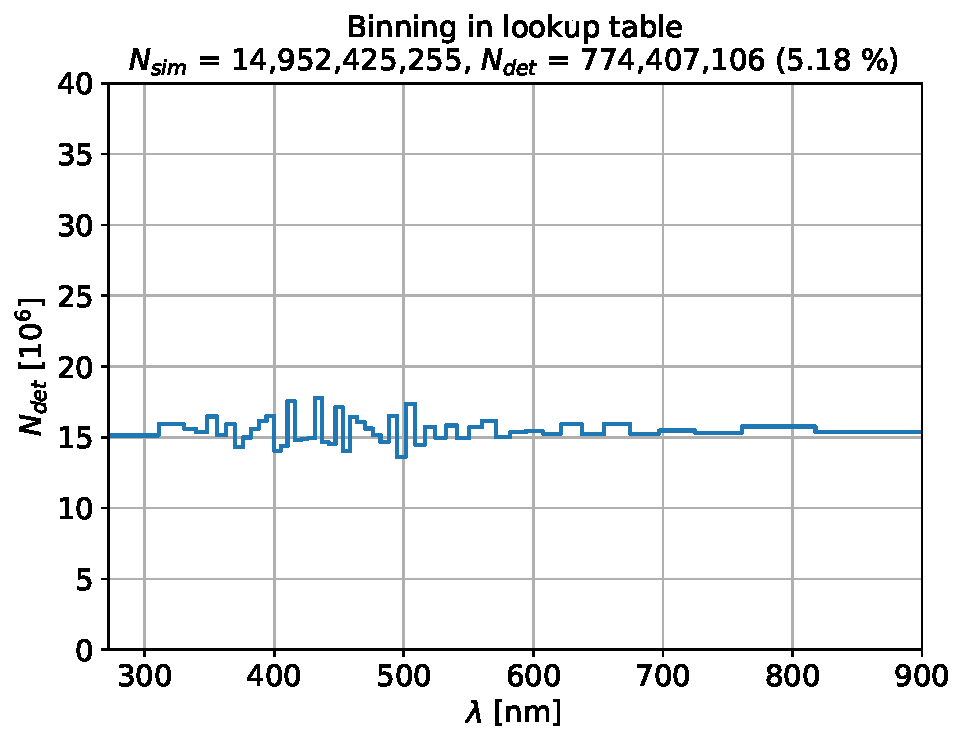
\includegraphics[width=\textwidth]{lut_wvl_bins_hist.pdf}
		\subcaption{adaptive binning}
		\label{param:wvl_binning:adaptive}
	\end{subfigure}
	\caption[Constant vs. adaptive wavelength binning]{\textbf{Constant vs. adaptive wavelength binning.} All wavelengths of photons that are detected by any camera SiPM are histogramized in \num{50} bins between \SI{272}{\nano\meter} and \SI{900}{\nano\meter}. In (\subref{param:wvl_binning:constant}), the \num{50} bins are distributed uniformly in wavelength so that one can see a shape that is quite similar to the PDE of the SiPMs. Figure~(\subref{param:wvl_binning:adaptive}) shows the same data with adaptive bin sizes to equalize the counts per bin. The resulting bin edges are rounded to integer numbers which causes the visible fluctuations. Since the adaptive bin limits are always included by closed intervals, there are slightly more detected photons in~(\subref{param:wvl_binning:adaptive}) than in~(\subref{param:wvl_binning:constant}) due to numerical issues. This is not a problem since also the simulated photons are binned in the same closed intervals which result in correct detection efficiency calculations.}
	\label{param:wvl_binning}
\end{figure}

The adaptive bin edges are calculated by sorting the wavelengths of all simulated particles that are detected by any of the 61 SiPM -- i.e. all photons on which the KDE will be applied afterwards (cf. section~\ref{sec:adaptive_vs_nonadaptive}). Next, this sequence is divided into \num{50} parts of equal length. Thus, the wavelengths are divided into consecutive \SI{2}{\percent}-quantiles. In order to get more convenient bin sizes, the quantile limits (or bin edges) are rounded to integer values which obviously result in some fluctuations (cf. figure~\ref{param:wvl_binning:adaptive}).

With the adaptive wavelength binning it is ensured that in each range $\Delta\lambda$ almost the same number of photons is detected which enables a statistically more stable probability density estimation. The simulated wavelength range starts at $\lambda_\text{min}=\SI{272}{\nano\meter}$ since there is no photon detected with a wavelength below \SI{272}{\nano\meter} due to the absorption properties or the glass plate (cf. \ref{sec:iceact:model:material}).

\section{Adaptive vs. Non-adaptive KDE}\label{sec:adaptive_vs_nonadaptive}

Now that the wavelength binning is defined, the next step is to take a look on the camera pixels individually. Due to the distinct field of view of each pixel, the direction distribution of each pixel is characteristic and has regions with very different statistical densities as already stated in section~\ref{sec:adaptive_kde}. In order to get an idea of the given direction distributions for which the KDE should be calculated, figure \ref{param:example_scatter} shows some exemplary scatter plots of detected photons by an arbitrary camera pixel~$i$ in a wavelength range~$\Delta\lambda$.\\

\begin{figure}[H]
	\centering
	\begin{subfigure}[t]{0.49\textwidth}
		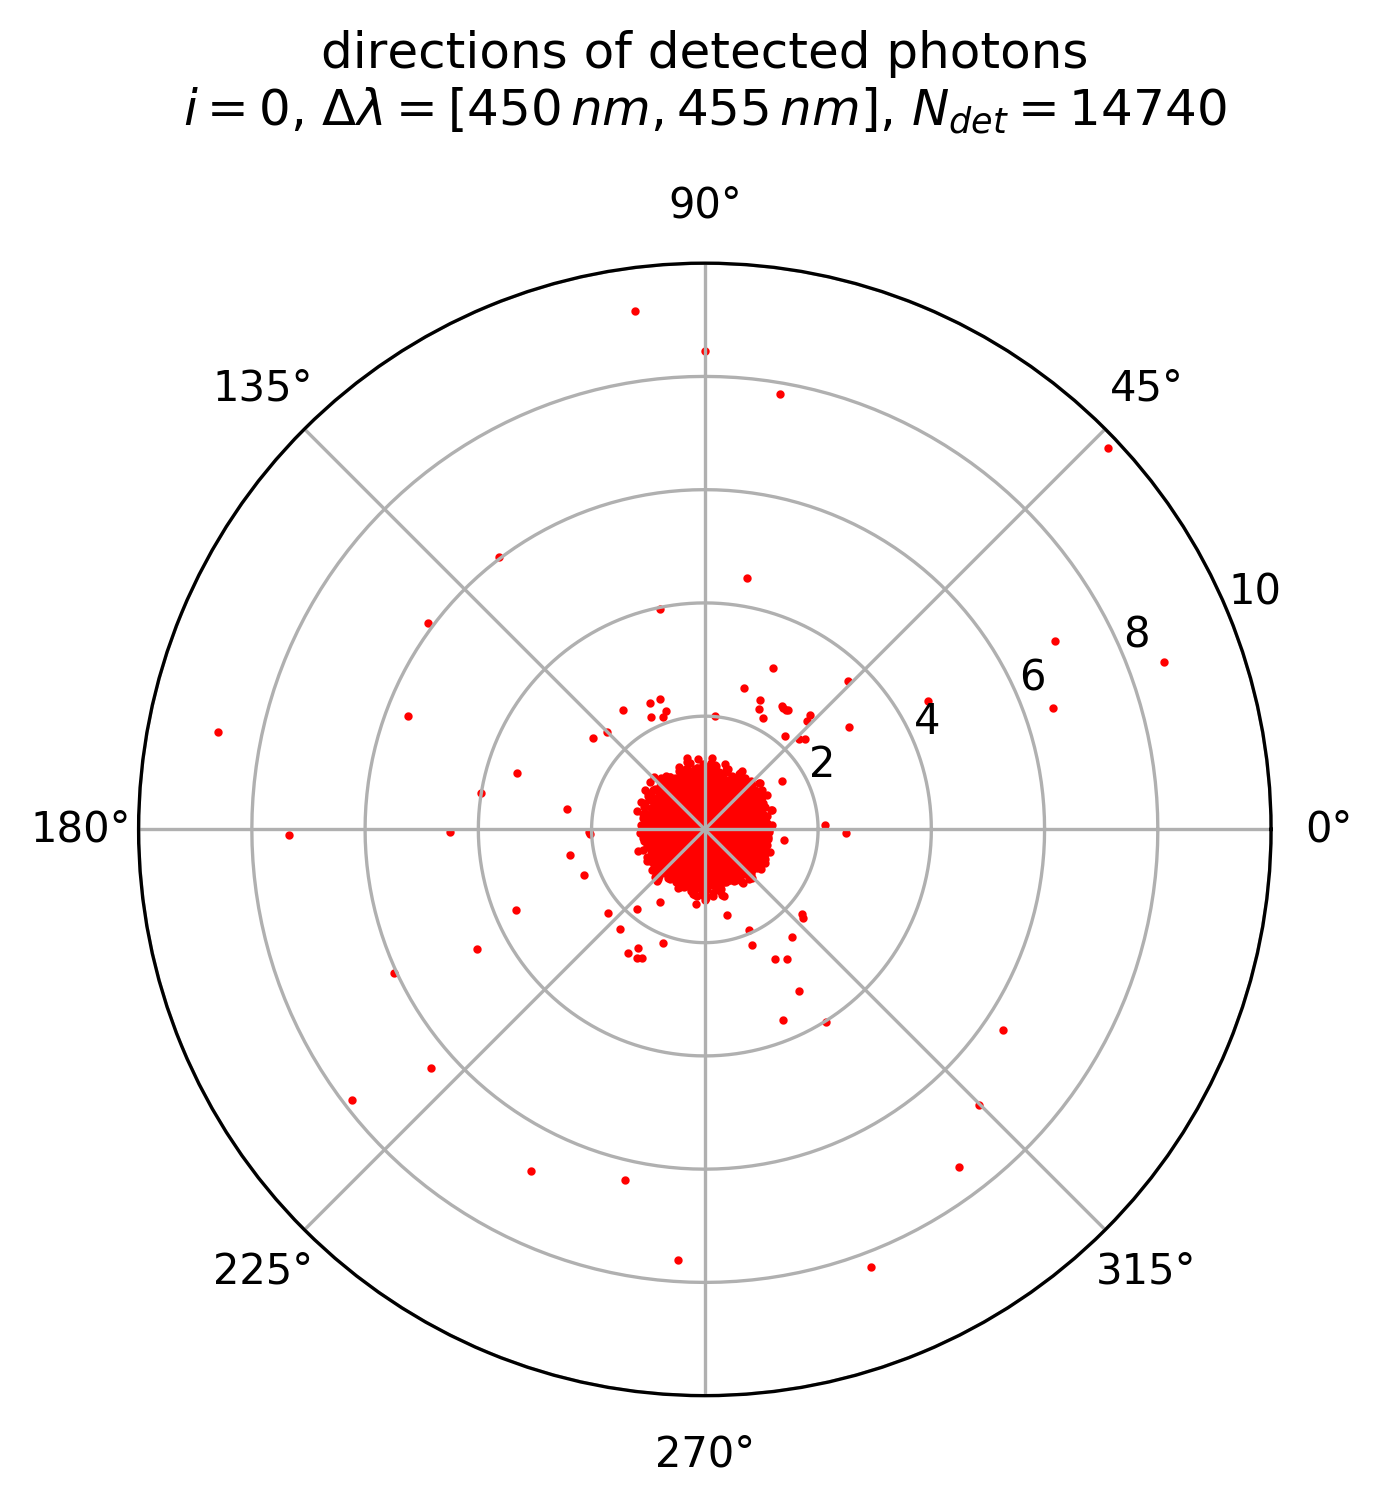
\includegraphics[width=\textwidth]{scatter_px00_wvl450-455nm.png}
		\subcaption{}
		\label{param:example_scatter:1}
	\end{subfigure}
	\hfill
	\begin{subfigure}[t]{0.49\textwidth}
		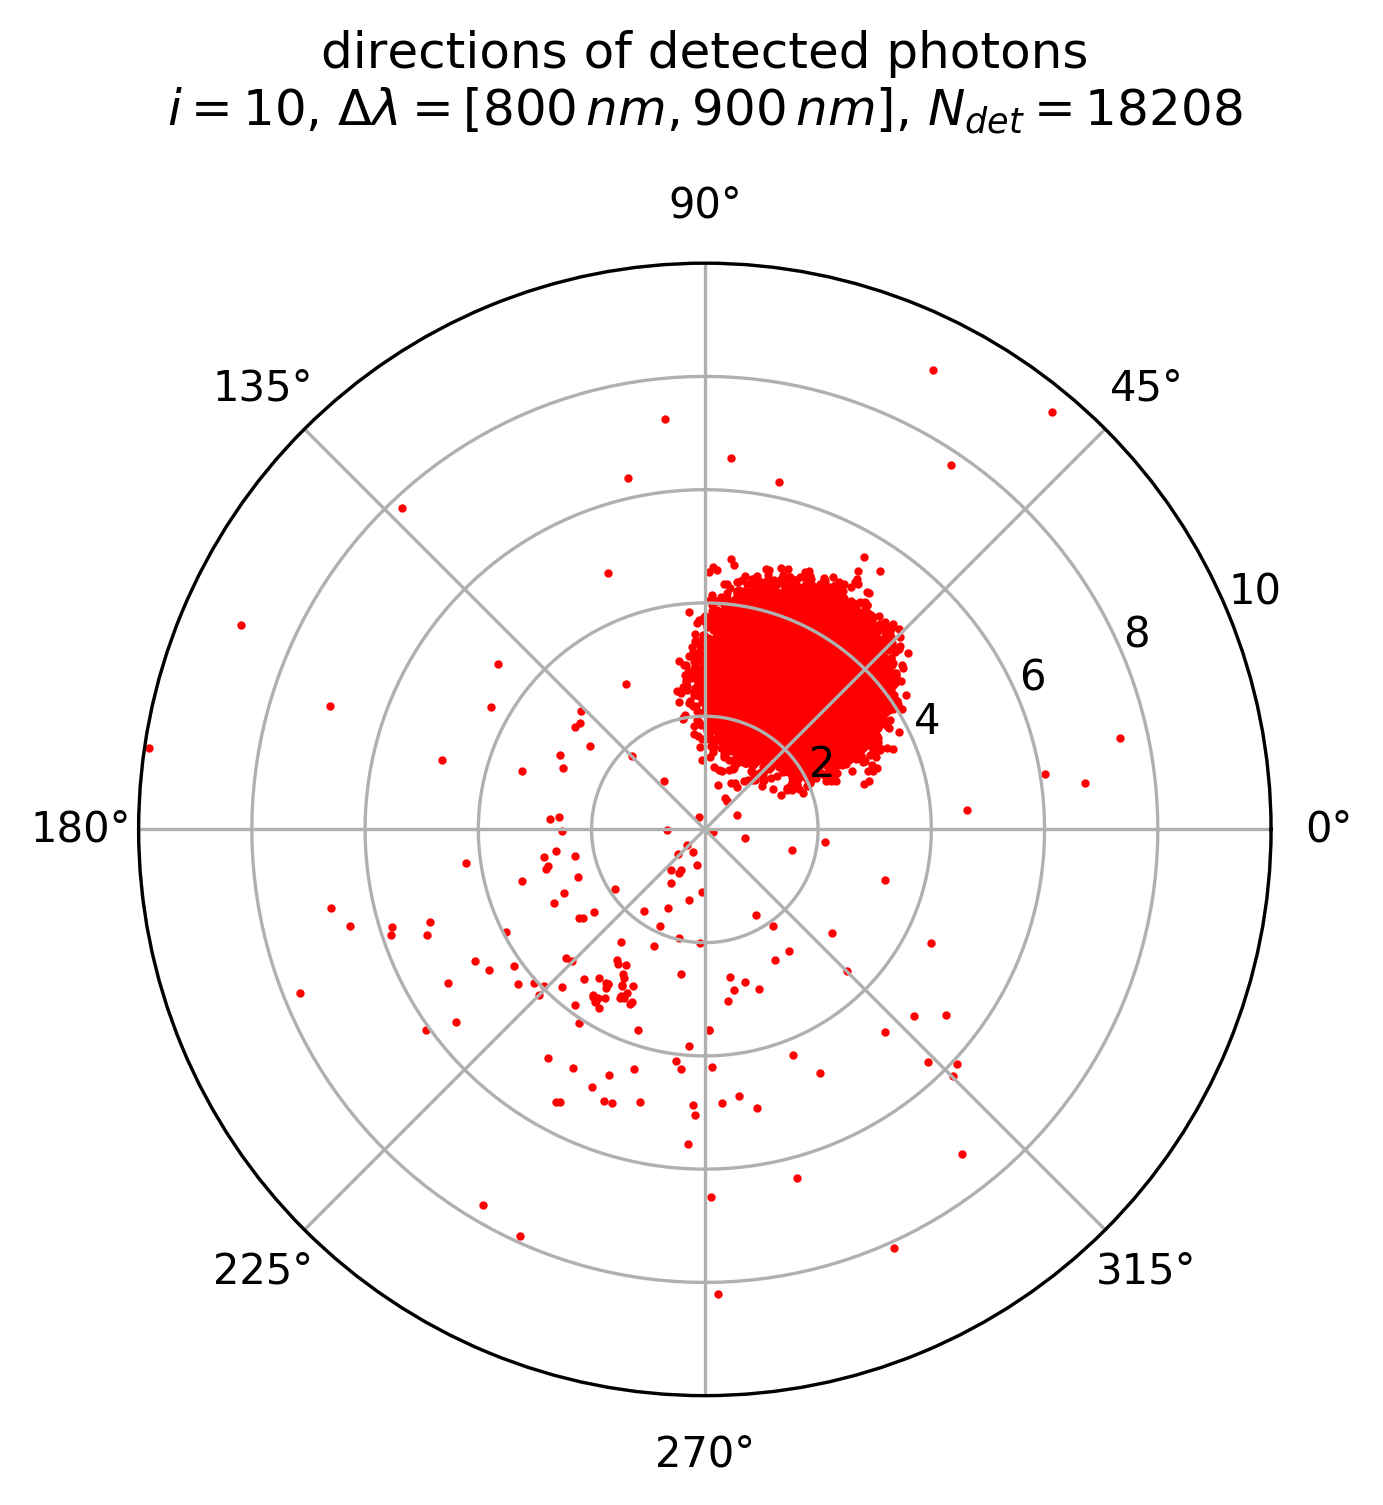
\includegraphics[width=\textwidth]{scatter_px10_wvl800-900nm.png}
		\subcaption{}
		\label{param:example_scatter:2}
	\end{subfigure}
	\vfill
	\begin{subfigure}[b]{0.49\textwidth}
		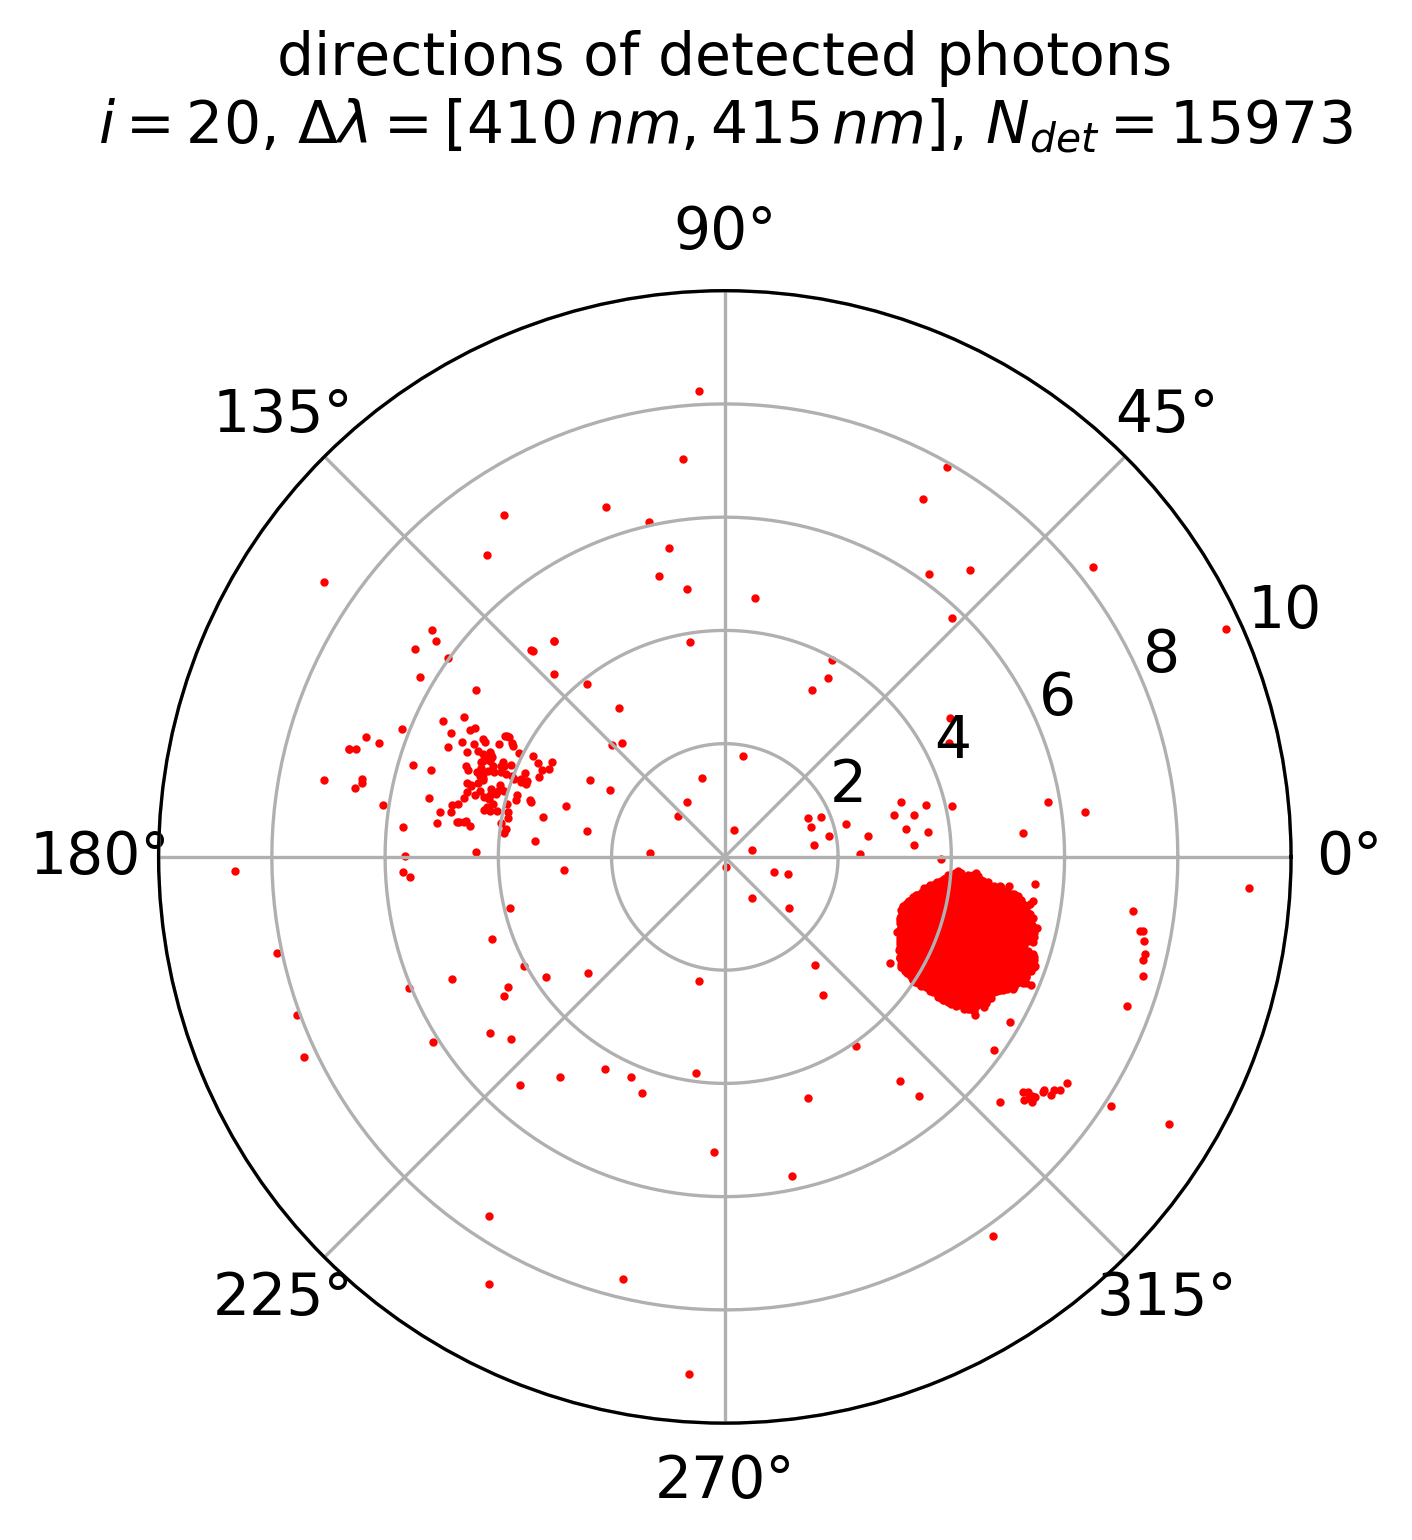
\includegraphics[width=\textwidth]{scatter_px20_wvl410-415nm.png}
		\subcaption{}
		\label{param:example_scatter:3}
	\end{subfigure}
	\hfill
	\begin{subfigure}[b]{0.49\textwidth}
		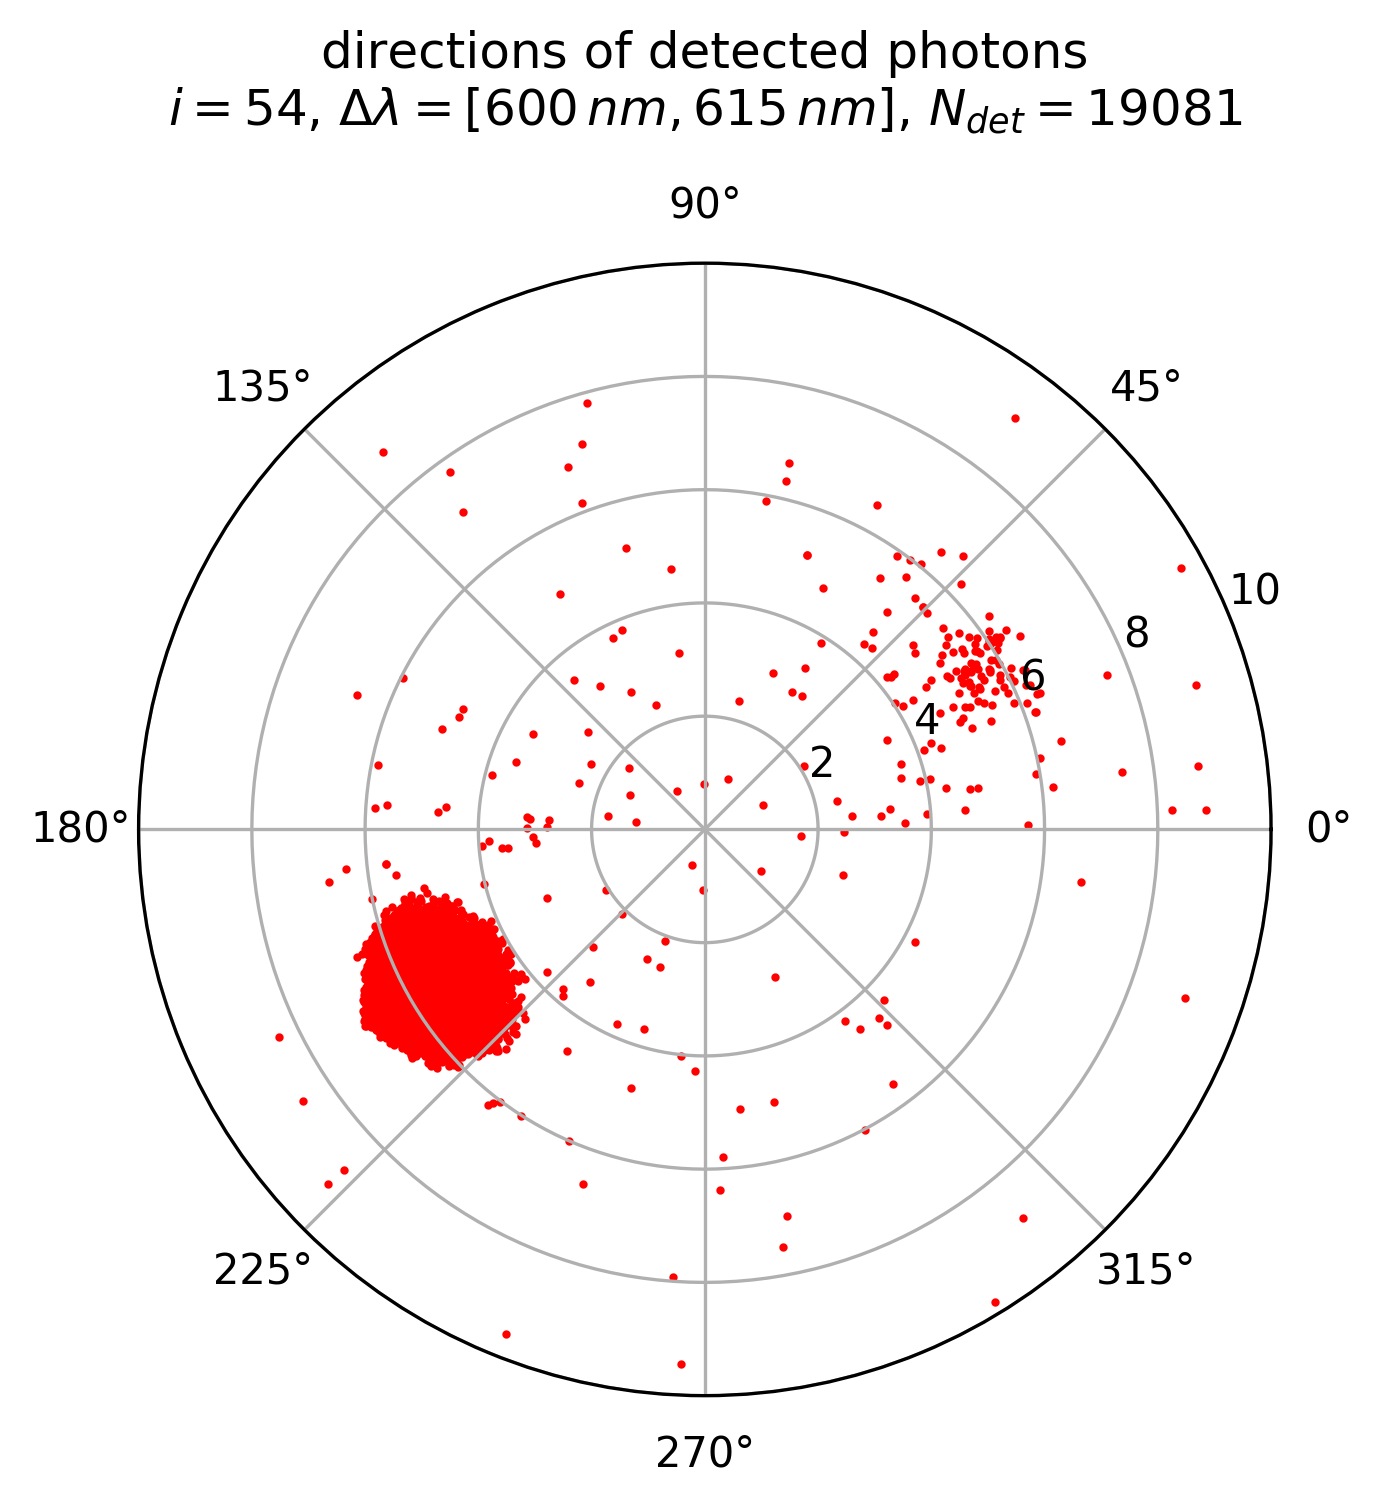
\includegraphics[width=\textwidth]{scatter_px54_wvl600-615nm.png}
		\subcaption{}
		\label{param:example_scatter:4}
	\end{subfigure}
	\caption[Example: directions of detected photons as a scatter plot]{\textbf{Example: directions of detected photons as a scatter plot.} A subset of simulated photon directions that are detected in a given camera pixel $i$ and the wavelength range $\Delta\lambda$ are shown in a polar plot. One can clearly see that there are regions with high and low statistical significance. Additionally, the \textit{ghost image} effect (cf. section~\ref{sec:ghost_image}) is visible in the non-central pixels ((\subref{param:example_scatter:2}), (\subref{param:example_scatter:3}), (\subref{param:example_scatter:4})).}
	\label{param:example_scatter}	
\end{figure}

The regions with very sparse \enquote{dots} can only arise from random scattering processes inside the optical system since they are outside the main field of view and the \textit{ghost image} region (cf. section~\ref{sec:ghost_image}). Thus, the probability density should be rather constant in these scattering regions. For the KDE, one achieves this by increasing the kernel bandwith. Simultaneously, the \enquote{real} detection regions should be described precisely which is done by reducing the bandwith. The need of an adaptive kernel density approach is given. Figure~\ref{param:kde_comparison} strikingly shows the difference between an adaptive and a non-adaptive KDE. Since the KDEs calculated there are only based on a small subsample of the simulation data, they may give the impression that the adaptive KDE still is very inaccurate in the scattering regions but on the full data sample this is not the case any more by having more scattered photons.\\

\begin{figure}[H]
	\centering
	\begin{subfigure}[t]{0.40\textwidth}
		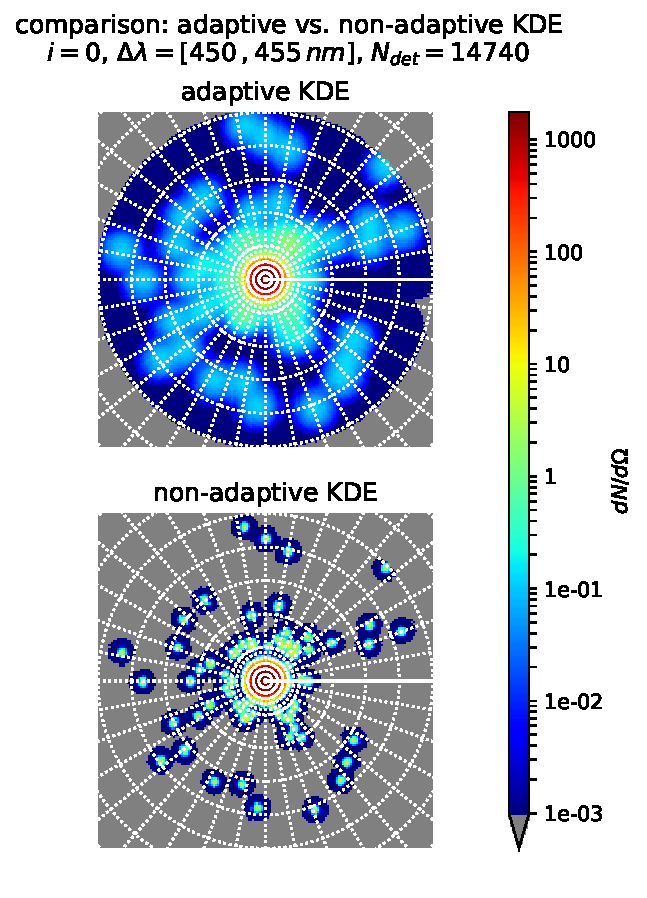
\includegraphics[width=\textwidth]{comparison_adaptive_nonadaptive_px00_wvl450-455.pdf}
		\subcaption{}
		\label{param:kde_comparison:1}
	\end{subfigure}
	\hfill
	\begin{subfigure}[t]{0.40\textwidth}
		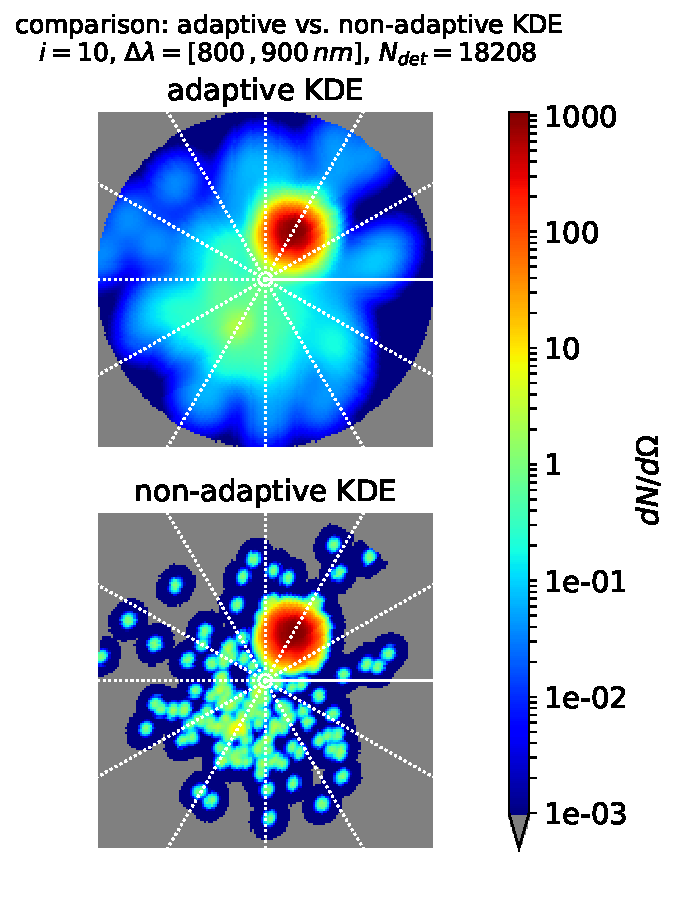
\includegraphics[width=\textwidth]{comparison_adaptive_nonadaptive_px10_wvl800-900.pdf}
		\subcaption{}
		\label{param:kde_comparison:2}
	\end{subfigure}
	\vfill
	\begin{subfigure}[b]{0.40\textwidth}
		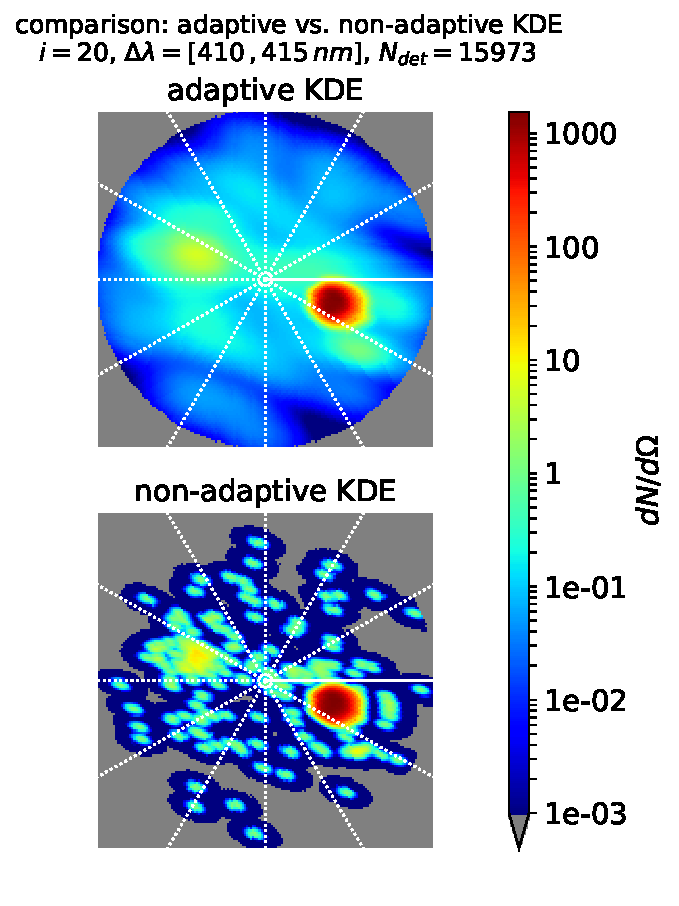
\includegraphics[width=\textwidth]{comparison_adaptive_nonadaptive_px20_wvl410-415.pdf}
		\subcaption{}
		\label{param:kde_comparison:3}
	\end{subfigure}
	\hfill
	\begin{subfigure}[b]{0.40\textwidth}
		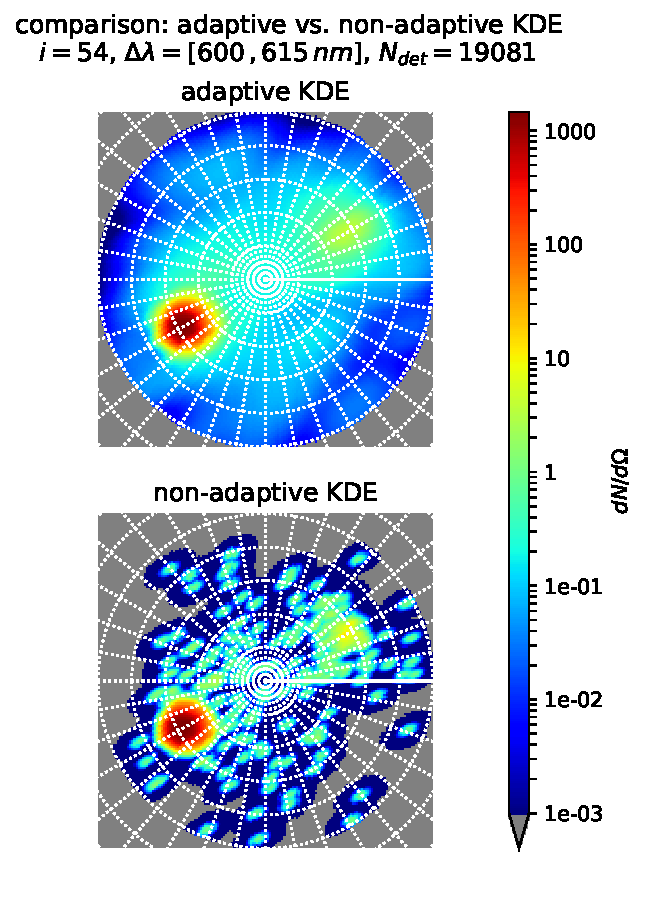
\includegraphics[width=\textwidth]{comparison_adaptive_nonadaptive_px54_wvl600-615.pdf}
		\subcaption{}
		\label{param:kde_comparison:4}
	\end{subfigure}
	\caption[Comparison: adaptive vs. non-adaptive KDE]{\textbf{Comparison: adaptive vs. non-adaptive KDE.} Evaluation of the direction distributions shown in figure~\ref{param:example_scatter} on a HEALPix grid with $N_\text{side}=\num{512}$. The plot shows a disc up to $\theta=\SI{10}{\degree}$ and the white dotted meridians have an azimuth distance of $\SI{30}{\degree}$. The azimuth $\phi$ starts at the solid white line and goes around counter-clockwise. Differences between an adaptive (top) and non-adaptive (bottom) KDE approach are visible. Especially in the region with low statistics (scattering region), the non-adaptive KDE is dominated by the fluctuations while adaptive KDE blurs the probability density more strongly.}
	\label{param:kde_comparison}		
\end{figure}

Anyway, the detection distributions can now be calculated and renormalized for each of the \num{61} camera pixels and \num{50} wavelength bins which result in \num{3050} so called \textit{detection efficiency maps} shown in the next section~\ref{sec:deteff_maps}.

\section{Detection Efficiency Maps}\label{sec:deteff_maps}

By following the strategy described in chapter~\ref{chap:param:strategy} and considering the findings from sections~\ref{sec:wvl_binning} and \ref{sec:adaptive_vs_nonadaptive}, one can now finally calculate \textit{detection efficiency maps}. For each camera pixel $i$ and wavelength bin $\Delta\lambda$, these maps show the probability $\epsilon_{i,\Delta\lambda,HP}$ to detect a photon with wavelength $\lambda\in\Delta\lambda$ in camera pixel $i$ as a function of its origin direction~$(\theta,\phi)$ which is coded in the ordinal number~$HP$ of the corresponding HEALPix. For the error estimation, the bootstrapping method presented in section~\ref{sec:bootstrapping} is used. To get a confident estimation with reasonable computational effort, $N_\text{bootstrap} = \num{10}$ bootstrapping iterations are performed.\\

\subsection{Choice of HEALPix Pixelization Parameter $N_\text{side}$}

For the pixelization parameter of the HEALPix model~$N_\text{side}$, one has to choose a reasonable value as well (cf. table~\ref{healpix:table}): too fine pixelization would obviously result in a very detailed parameterization. Due to KDE, an \enquote{unbinned} detection efficiency is available -- at least in origin directions -- so that it is technically possible to choose a very fine binning. The problem is, that the main goal of the \iceact parameterization is to produce a lookup table that is efficient and capable of evaluating large amounts of Cherenkov photons. An unnecessarily fine HEALPix binning would just blow up the lookup table and quick evaluation is not feasible anymore. To determine the optimal $N_\text{side}$ of the HEALPix model, the detection efficiency of the central pixel $i=0$ is considered. As one can see in figure~\ref{deteffmap:px0}, the most efficient angular area is below a zenith angle of $\theta=\SI{0.7}{\degree}$. Usually, this regions are called \textit{field of view} (\textit{FOV}) which equals the doubled zenith angle $2\theta$ if the FOV is symmetrical around the zenith. Thus, the core field of view of the central pixel is $\SI{1.4}{\degree}$. In the transition region $\SI{1.4}{\degree} < 2\theta \leq \SI{2.5}{\degree}$, the detection efficiency decreases rapidly. Therefore, is it crucial to pixelize this region such that the hexagonal shape of the pixel's field of view -- which is caused by the Winston cones -- is described in a sufficient degree of detail in order to have a fairly precise approximation.

\begin{figure}[H]
	\centering
	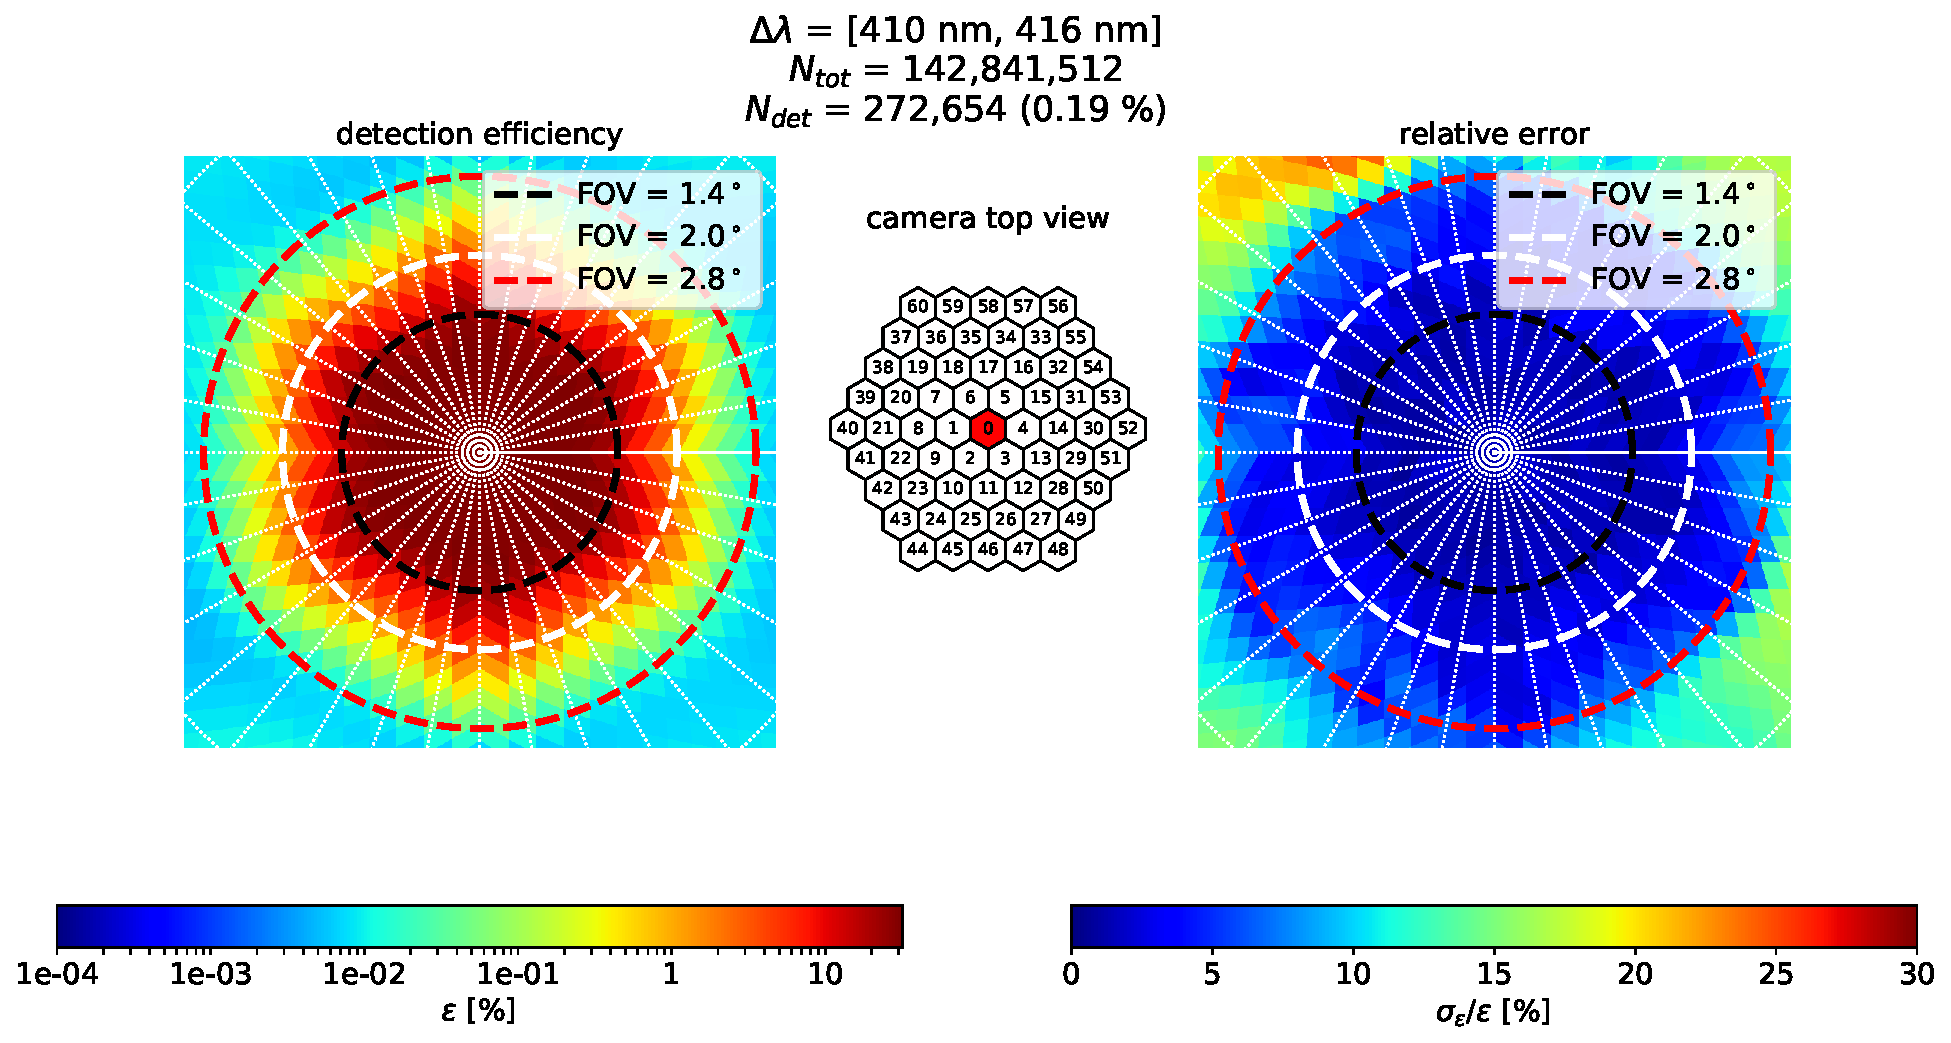
\includegraphics[width=\textwidth]{deteffmaps/deteff_wvl413nm_px00_view1.5deg.pdf}
	\caption[Detection efficiency of central camera pixel]{\textbf{Detection efficiency of central camera pixel.} The plot is zoomed into the main detection region up to a zenith angle $\theta=\SI{1.5}{\degree}$. As a wavelength, the bin around the most efficient wavelength~$\lambda^\ast$ (cf. section~\ref{sec:best_wvl}) is chosen. In a field of view below $\SI{1.4}{\degree}$, the central pixel has its maximal detection efficiency. The HEALPix parameter in this map is $N_\text{side}=\num{512}$. Bootstrapping leads to the relative error shown in the right plot. The interval between the white dashed meridians is $\Delta\phi=\SI{10}{\degree}$.}
	\label{deteffmap:px0}
\end{figure}

As figure~\ref{deteffmap:px0} shows, a HEALPix parameter of $N_\text{side}=\num{512}$ is sufficient to describe the hexagonal shape. By applying $N_\text{side}=\num{256}$, four HEALPix would reduce to just one HEALPix, which could hardly describe the edges. On the other side, one gets to $N_\text{side}=\num{1024}$ by dividing a HEALPix into four. This results in a unnecessarily high amount of HEALPix to describe the given shape. Table~\ref{n_healpix_fov} shows the number of enclosed HEALPix(-centers) in the core region ($2\theta\leq\SI{1.4}{\degree}$) and the transition region ($\SI{1.4}{\degree} < 2\theta \leq \SI{2.5}{\degree}$) depending on the used HEALPix parameter.

\begin{table}[H]
	\centering
	\begin{tabular}{c|c|c}
		\toprule
		\multirow{2}{*}{$N_\text{side}$} & \multicolumn{2}{c}{HEALPixes in region} \\
		&	$2\theta\leq\SI{1.4}{\degree}$ & $\SI{1.4}{\degree} < 2\theta \leq \SI{2.5}{\degree}$ \\
		\midrule
		\num{256}  & \num{24}  & \num{88} \\
		\num{512}  & \num{112} & \num{368} \\
		\num{1024} & \num{480} & \num{1380} \\
		\bottomrule
	\end{tabular}
	\caption[Number of HEALPixes centers in regions around the zenith]{\textbf{Number of HEALPixes centers in regions around the zenith.} The numbers for three possible HEALPix models are shown. As characteristic areas, the efficiency core region ($2\theta\leq\SI{1.4}{\degree}$) and transition region ($\SI{1.4}{\degree} < 2\theta \leq \SI{2.5}{\degree}$) of the central pixel around the most efficient wavelength~$\lambda^\ast$ (cf. section~\ref{sec:best_wvl}) are chosen.}
	\label{n_healpix_fov}
\end{table}

\subsection{Overview of Results}

In this section, some results are presented. At first, the focus is on the maximum detection efficiency. Just because the optics has been optimized to the \enquote{best} wavelength $\lambda^\ast=\SI{411}{\nano\meter}$ by minimizing the focal spot for this wavelength (cf. section~\ref{sec:focalplaneshift}), this does not necessarily imply that the detection efficiency is maximal at $\lambda^\ast$. Indeed, the maximal efficiency is reached between \SI{426}{\nano\meter} and \SI{431}{\nano\meter} for the central camera pixel with $\epsilon_\text{max}\approx\SI{33.35}{\percent}$ as figure~\ref{max_deteff} shows. One also observes, that for the off-axis pixels -- i.e. all but the central one -- the centroid of the efficiency distributions slightly shifts towards higher wavelengths which. The reason is that the focal plane shifts \enquote{behind} the camera plane with increasing wavelengths (cf. figure~\ref{focalplaneshift}). The higher the wavelength, the more blurred the image gets and these wavelengths are tendentially seen by more pixels. As a result, more inner pixels are more sensitive to lower and more outer pixels are more sensitive to higher wavelengths.\\

\begin{figure}[H]
	\centering
	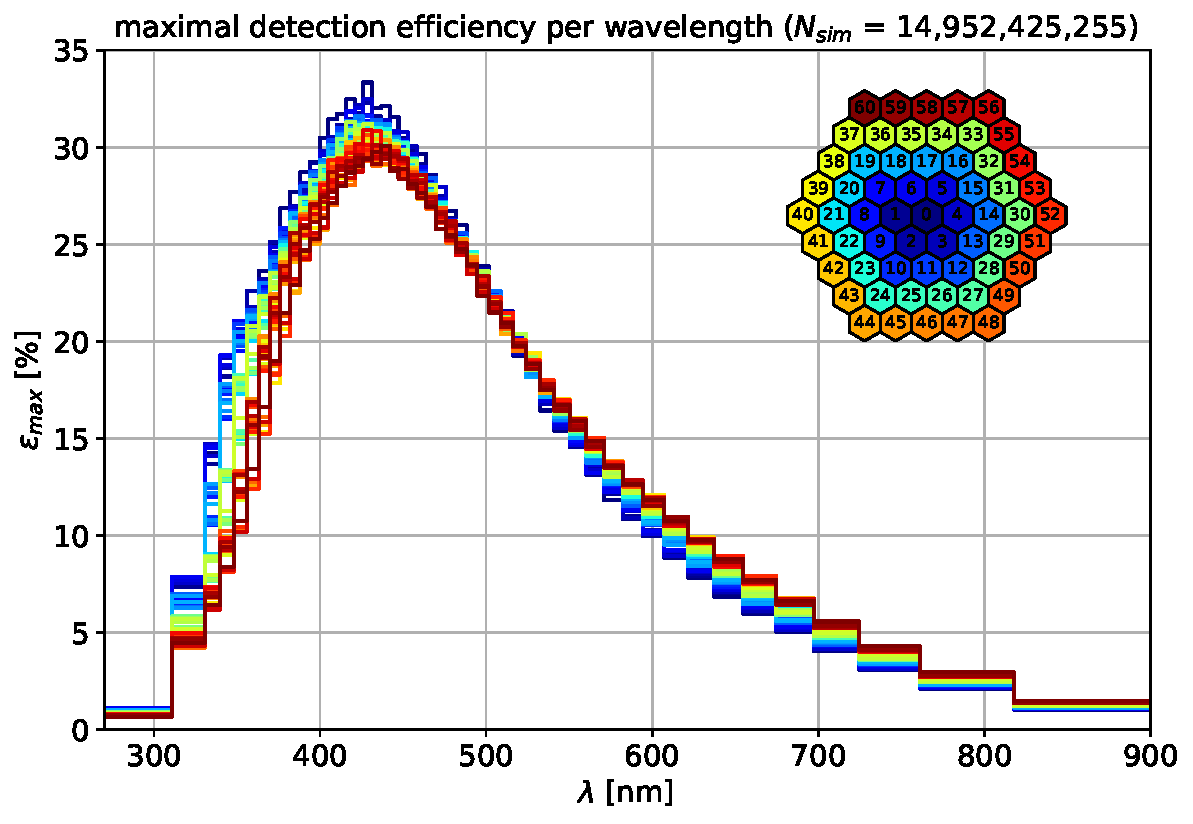
\includegraphics[width=0.7\textwidth]{deteffmaps/deteff_bins_max.pdf}
	\caption[Maximum detection efficiency for each pixel and wavelength]{\textbf{Maximum detection efficiency for each pixel and wavelength.} The 61 camera pixels are color-coded via their ordinal number from blue to read. The overall maximum detection efficiency is reached by the central pixel at $\Delta\lambda=[\SI{426}{\nano\meter},\SI{431}{\nano\meter}]$ with $\epsilon_\text{max}\approx\SI{33.35}{\percent}$.}
	\label{max_deteff}
\end{figure}

By summing up the individual detection efficiency maps of each pixel, the response of the whole camera to a certain wavelength is given. Figure~\ref{deteff:full_cam} shows these maps for three characteristic wavelength ranges. What is remarkable is that in the region of focus, i.e. wavelengths for which the focal spot on the camera plane is relatively small, the geometry of the camera is important. One can see very sharp differences between the main field of view of each pixel which corresponds to the Winston cone centers and the Winston cone edges resulting in an approximately \SI{10}{\percent} lower efficiency (cf. figure~\ref{deteff:full_cam:2}). For smaller wavelengths where the focus is above the camera plane, a distinct geometry-dependent pattern is not visible except, of course, the overall hexagonal shape. For higher wavelengths, a pattern is again visible, but a barrel-shaped distortion is visible. This is a known optical aberration effect where the magnification decreases with distance from the optical axis like for an image of a fisheye lens.\\

\begin{figure}[H]
	\centering
	\begin{subfigure}[t]{0.705\textwidth}
		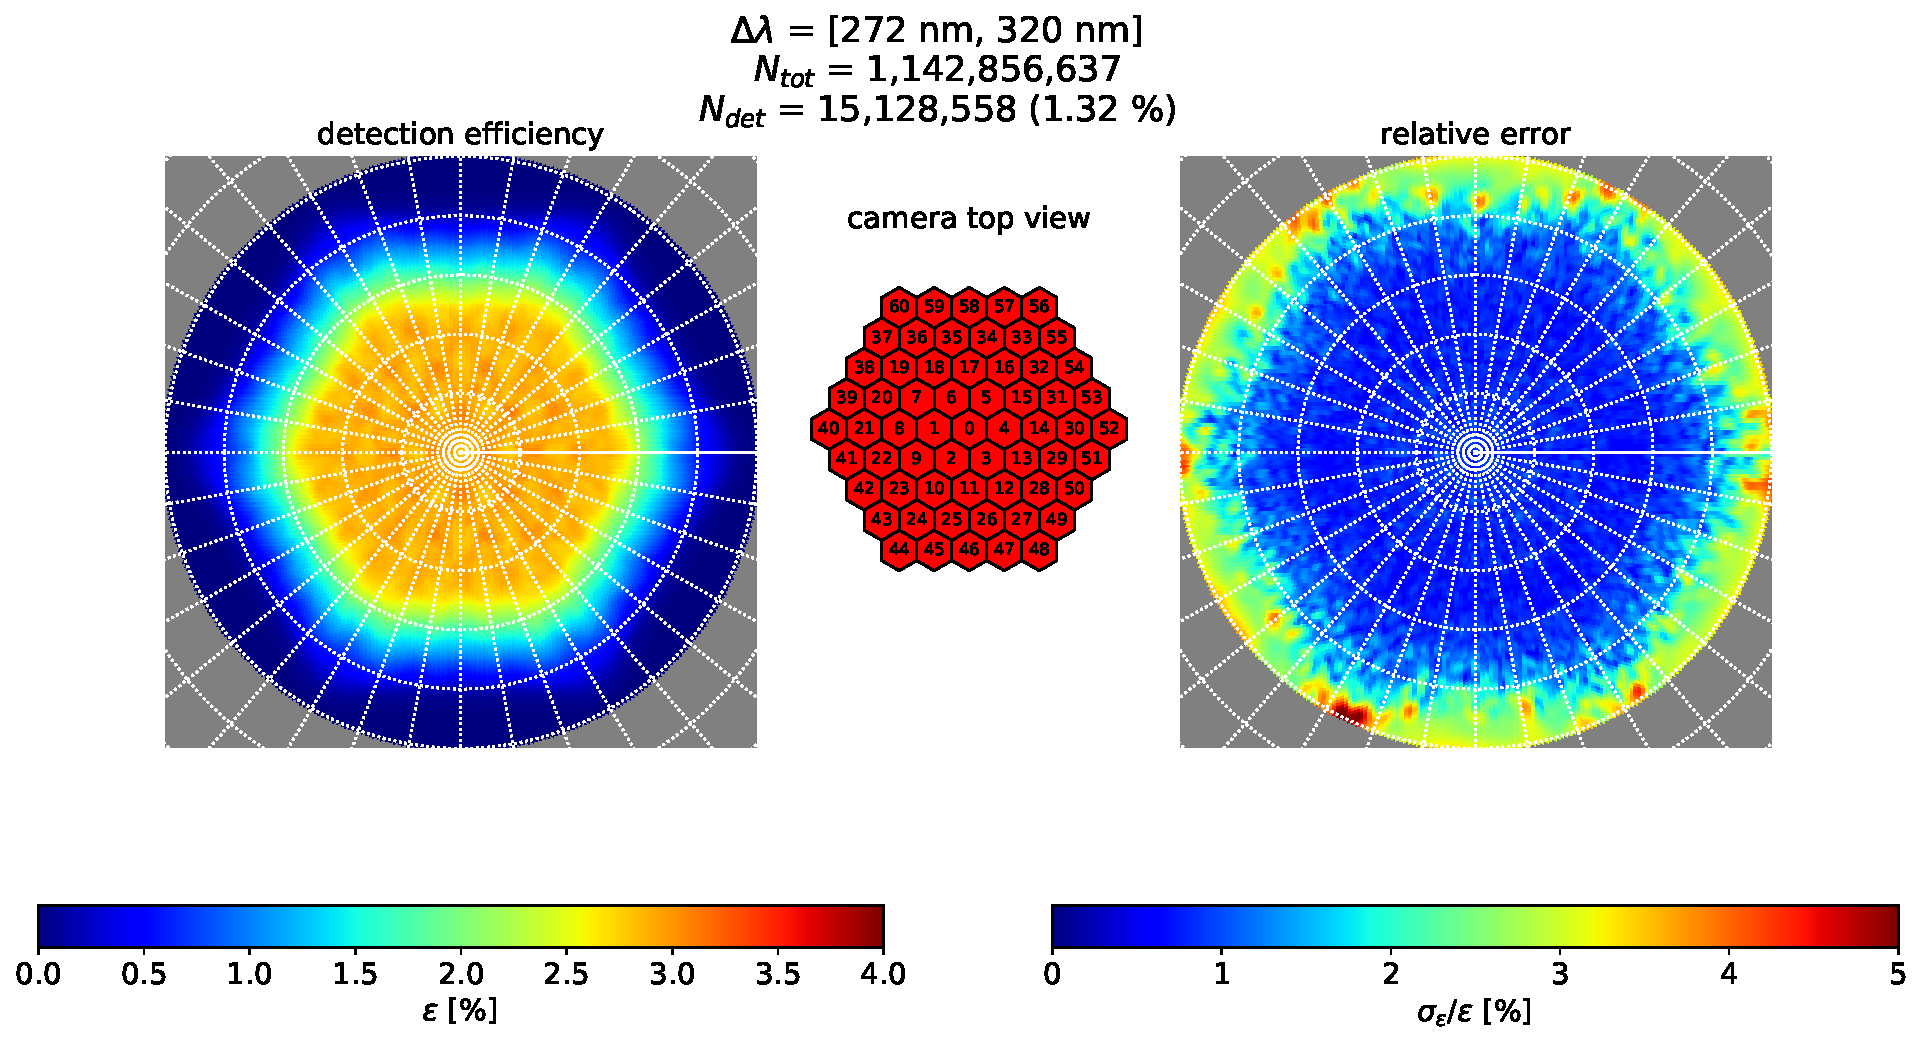
\includegraphics[width=\textwidth]{deteffmaps/deteff_wvl296nm_pxall_view10deg.pdf}
		\subcaption{Ultra-violet range.}
		\label{deteff:full_cam:1}
	\end{subfigure}
	\hfill
	\begin{subfigure}[t]{0.705\textwidth}
		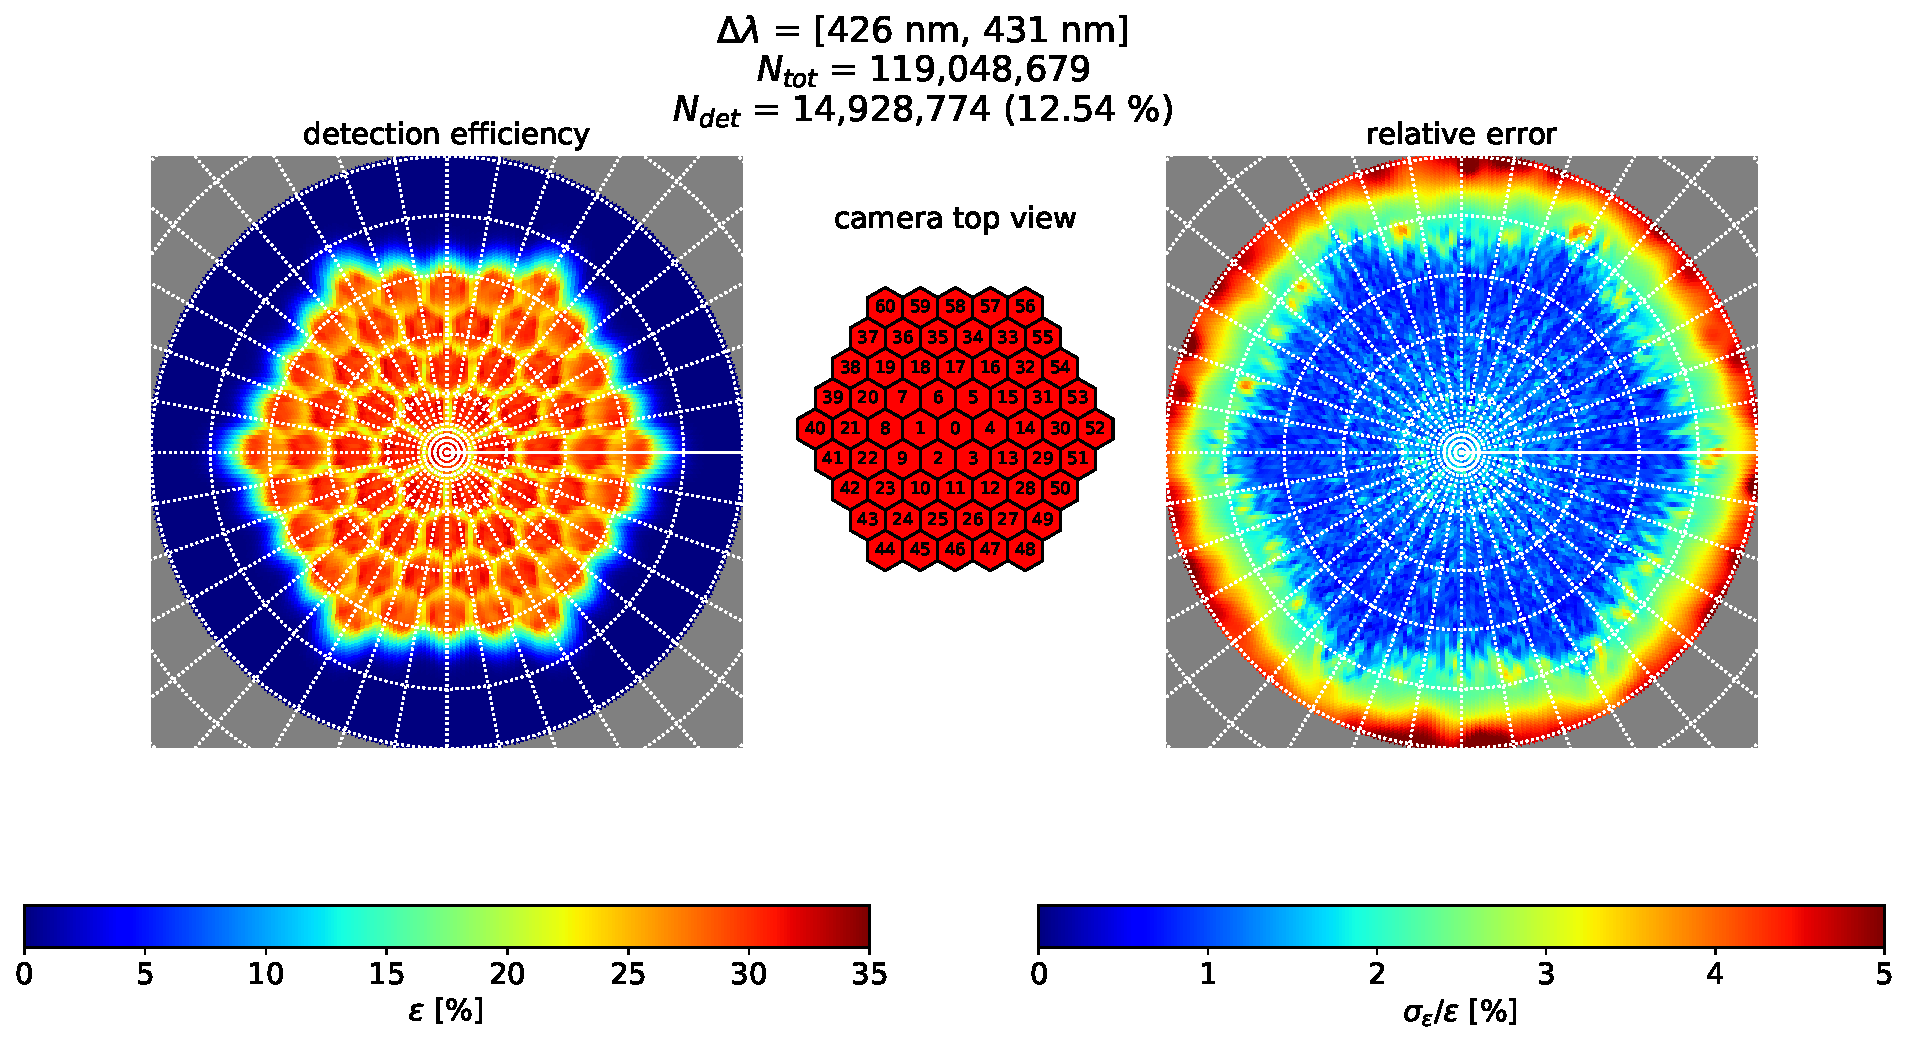
\includegraphics[width=\textwidth]{deteffmaps/deteff_wvl428.5nm_pxall_view10deg.pdf}
		\subcaption{Maximal efficient range.}
		\label{deteff:full_cam:2}
	\end{subfigure}
	\vfill
	\begin{subfigure}[t]{0.705\textwidth}
		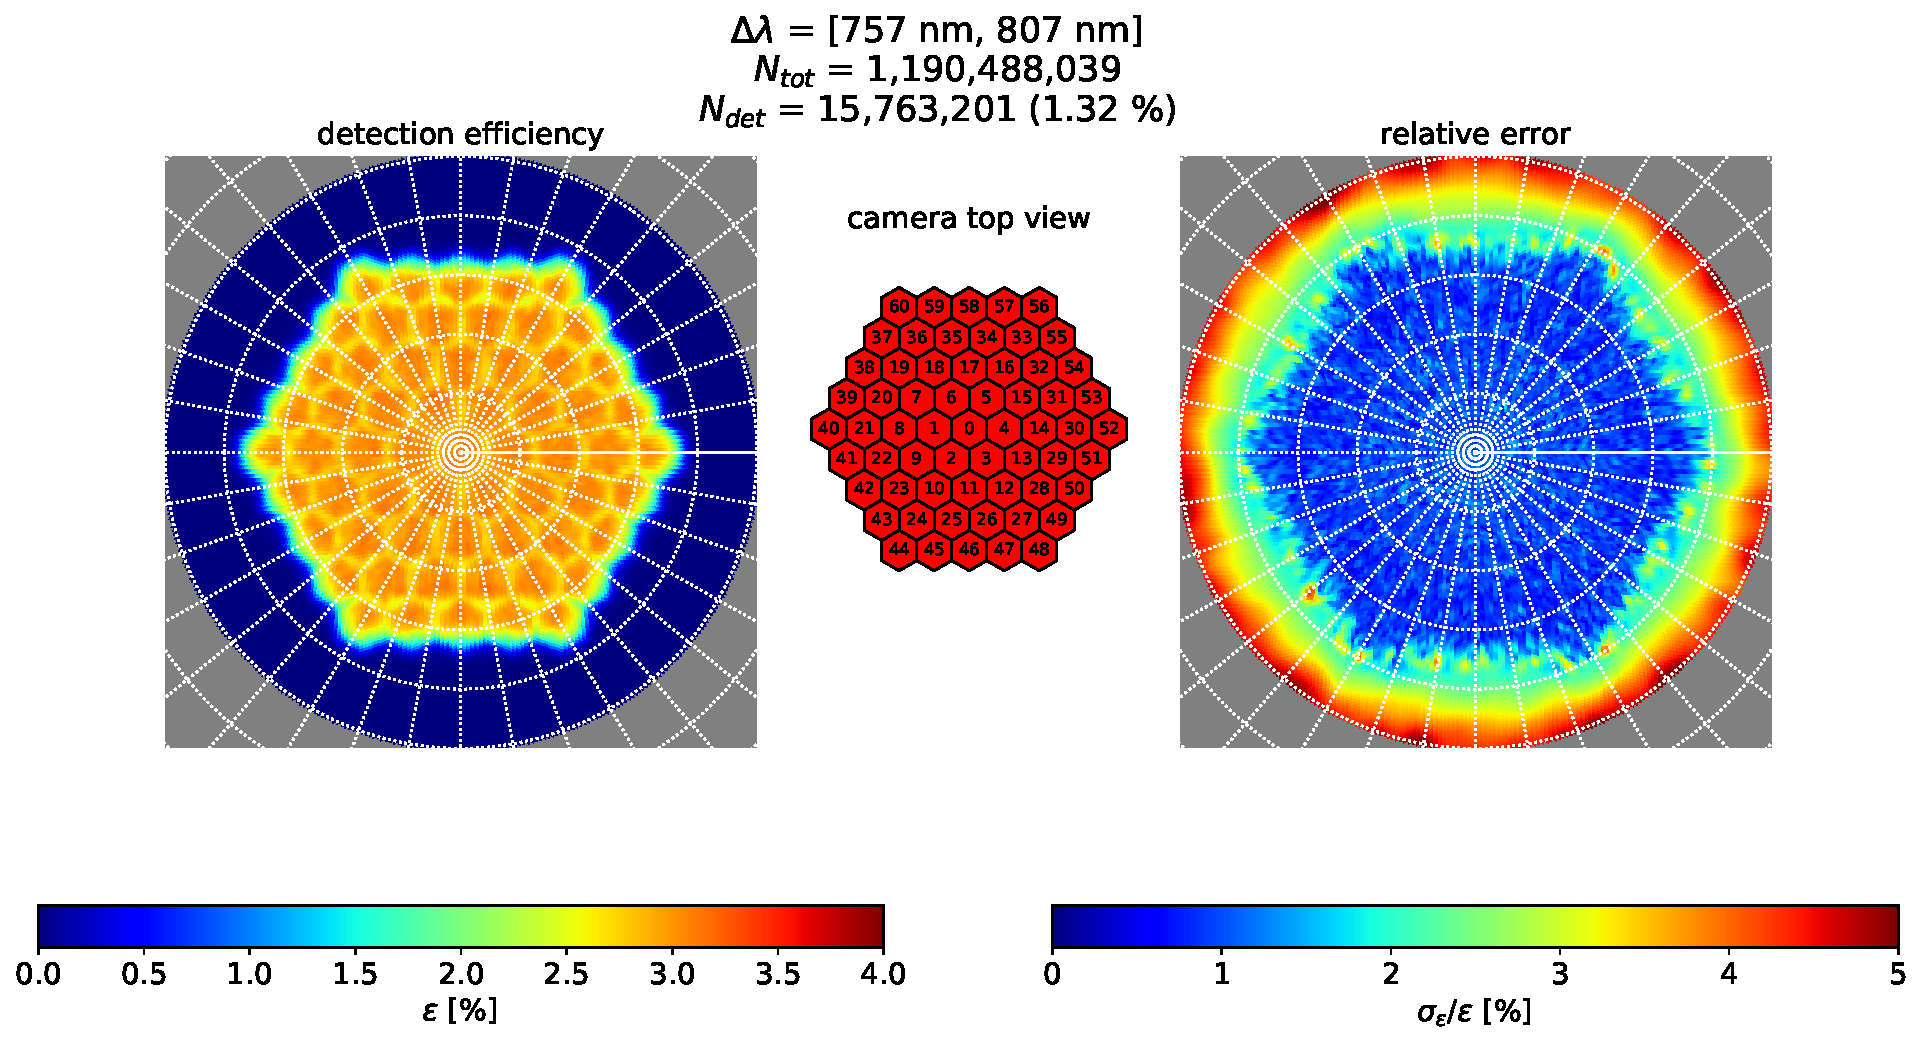
\includegraphics[width=\textwidth]{deteffmaps/deteff_wvl782nm_pxall_view10deg.pdf}
		\subcaption{High wavelengths range.}
		\label{deteff:full_cam:3}
	\end{subfigure}
	\caption[Detection efficiency maps of the full camera]{\textbf{Detection efficiency maps of the full camera.} The left plots show the detection efficiency while the right plots show the relative error. Three wavelength regions are chosen: a UV range in (\subref{deteff:full_cam:1}), the maximum efficiency in (\subref{deteff:full_cam:2}) and high wavelengths in (\subref{deteff:full_cam:3}). The white dashed parallels and meridians have the distances $\Delta\theta=\SI{2}{\degree}$ and $\Delta\phi=\SI{10}{\degree}$. The azimuth revolves counter-clockwisely starting at the white solid line. Please note the different color mapping for the detection efficiencies.}
	\label{deteff:full_cam}		
\end{figure}

Interesting optical effects are visible if one plots some off-axis pixels individually. Figure~\ref{deteff:offaxis_px} shows three of these. Besides the core region one can also see the ghost image explained in section~\ref{sec:ghost_image} on the opposide side in terms of the azimuth. Additionally, there are some spots next to the core and the ghost image region which originate from reflections between the Winston cones' top and Fresnel lens' back side. In blind regions where the detection probability does not exceed \SI{e-3}{\percent}, the estimated efficiency is highly dominated by statistical fluctuations as the plots for relative statistical errors show as well.\\

\begin{figure}[H]
	\centering
	\begin{subfigure}[t]{0.705\textwidth}
		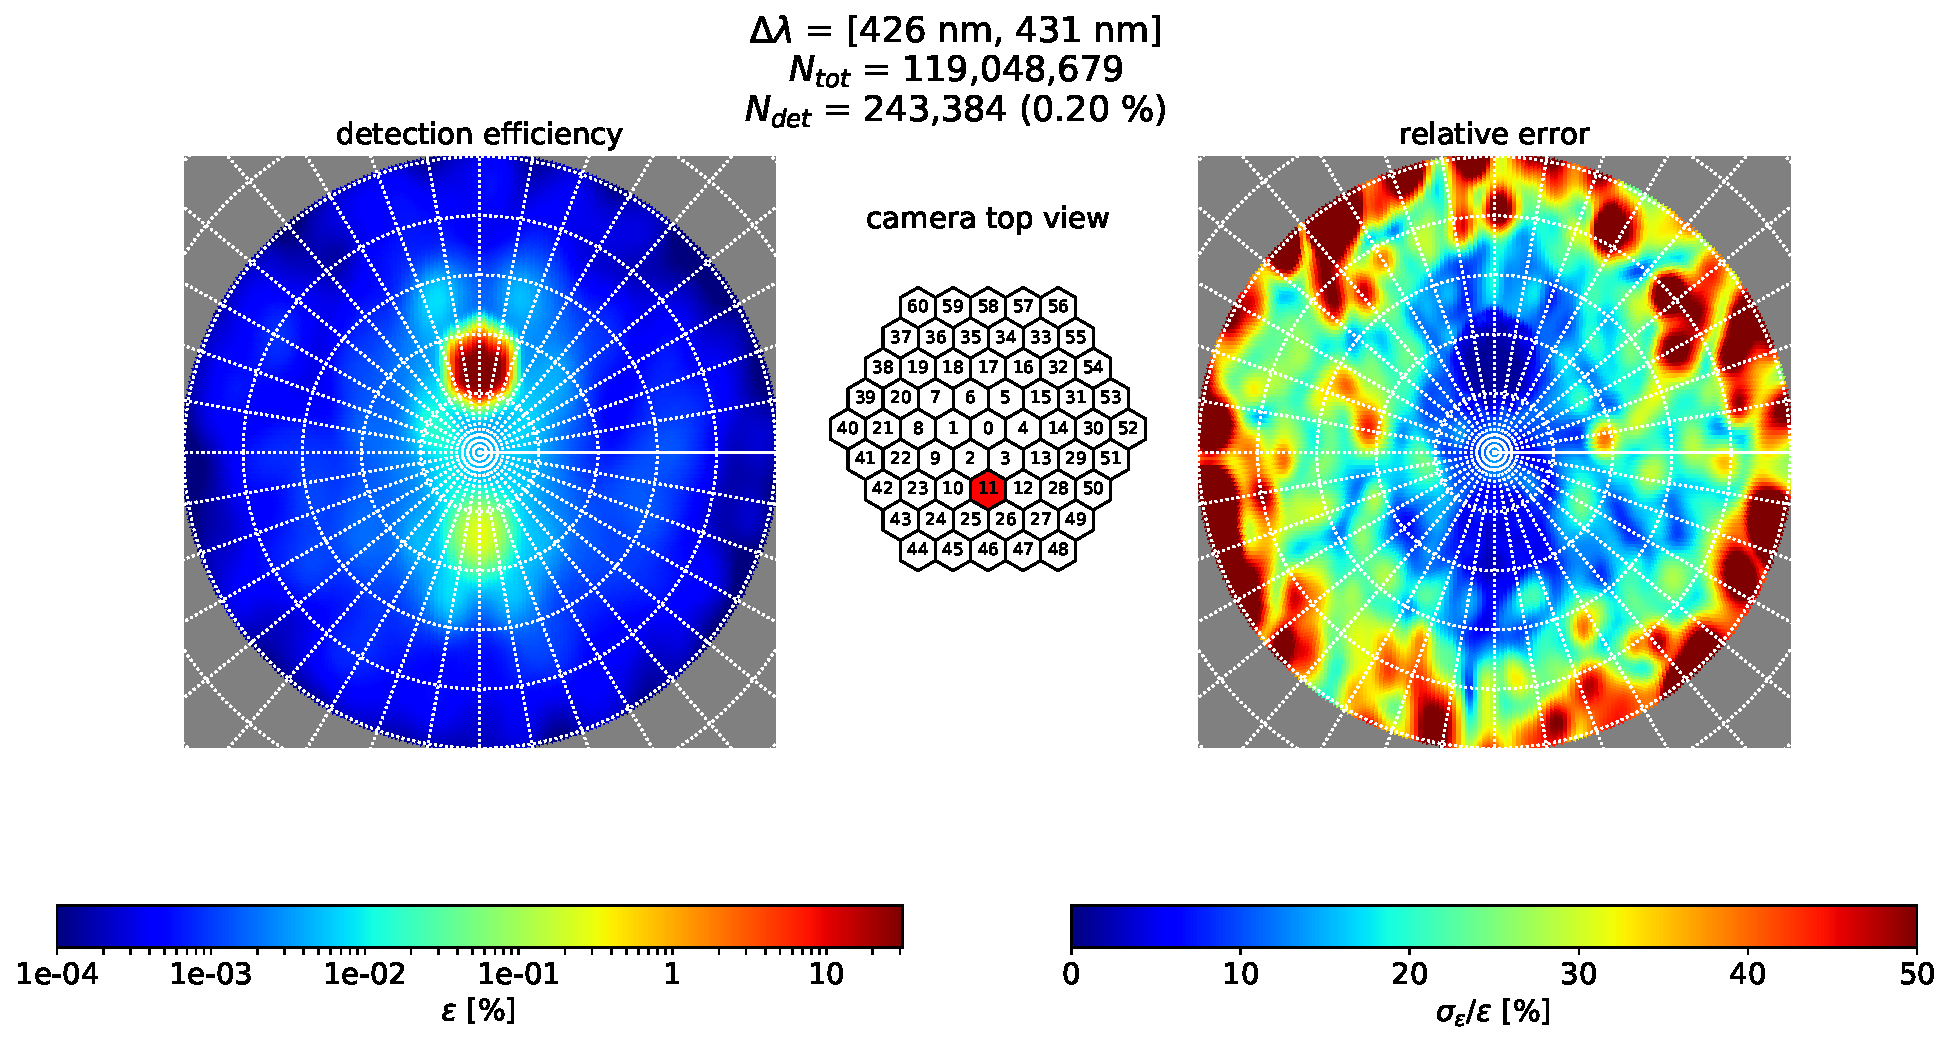
\includegraphics[width=\textwidth]{deteffmaps/deteff_wvl428.5nm_px11_view10.0deg.pdf}
		\subcaption{Pixel 11 on symmetry axis along $y$.}
		\label{deteff:offaxis_px:1}
	\end{subfigure}
	\hfill
	\begin{subfigure}[t]{0.705\textwidth}
		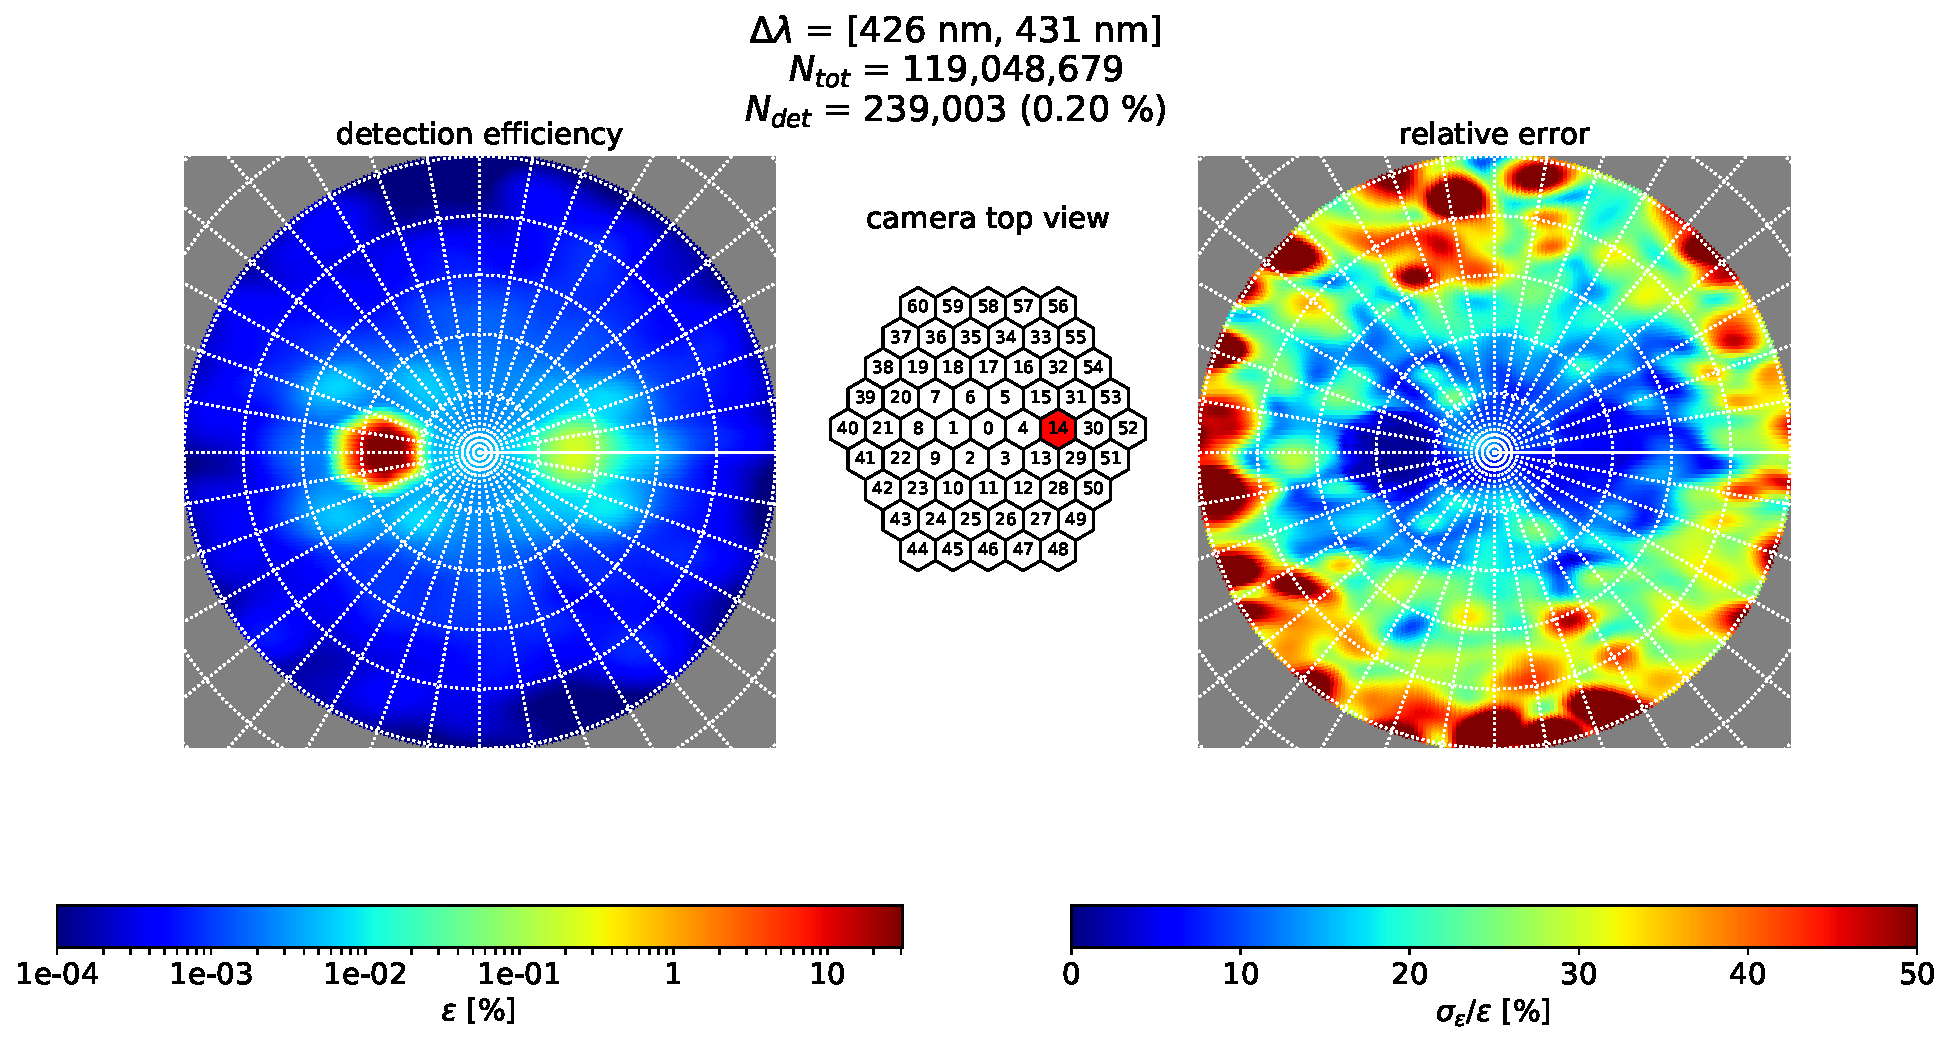
\includegraphics[width=\textwidth]{deteffmaps/deteff_wvl428.5nm_px14_view10.0deg.pdf}
		\subcaption{Pixel 14 on symmetry axis along $x$.}
		\label{deteff:offaxis_px:2}
	\end{subfigure}
	\vfill
	\begin{subfigure}[t]{0.705\textwidth}
		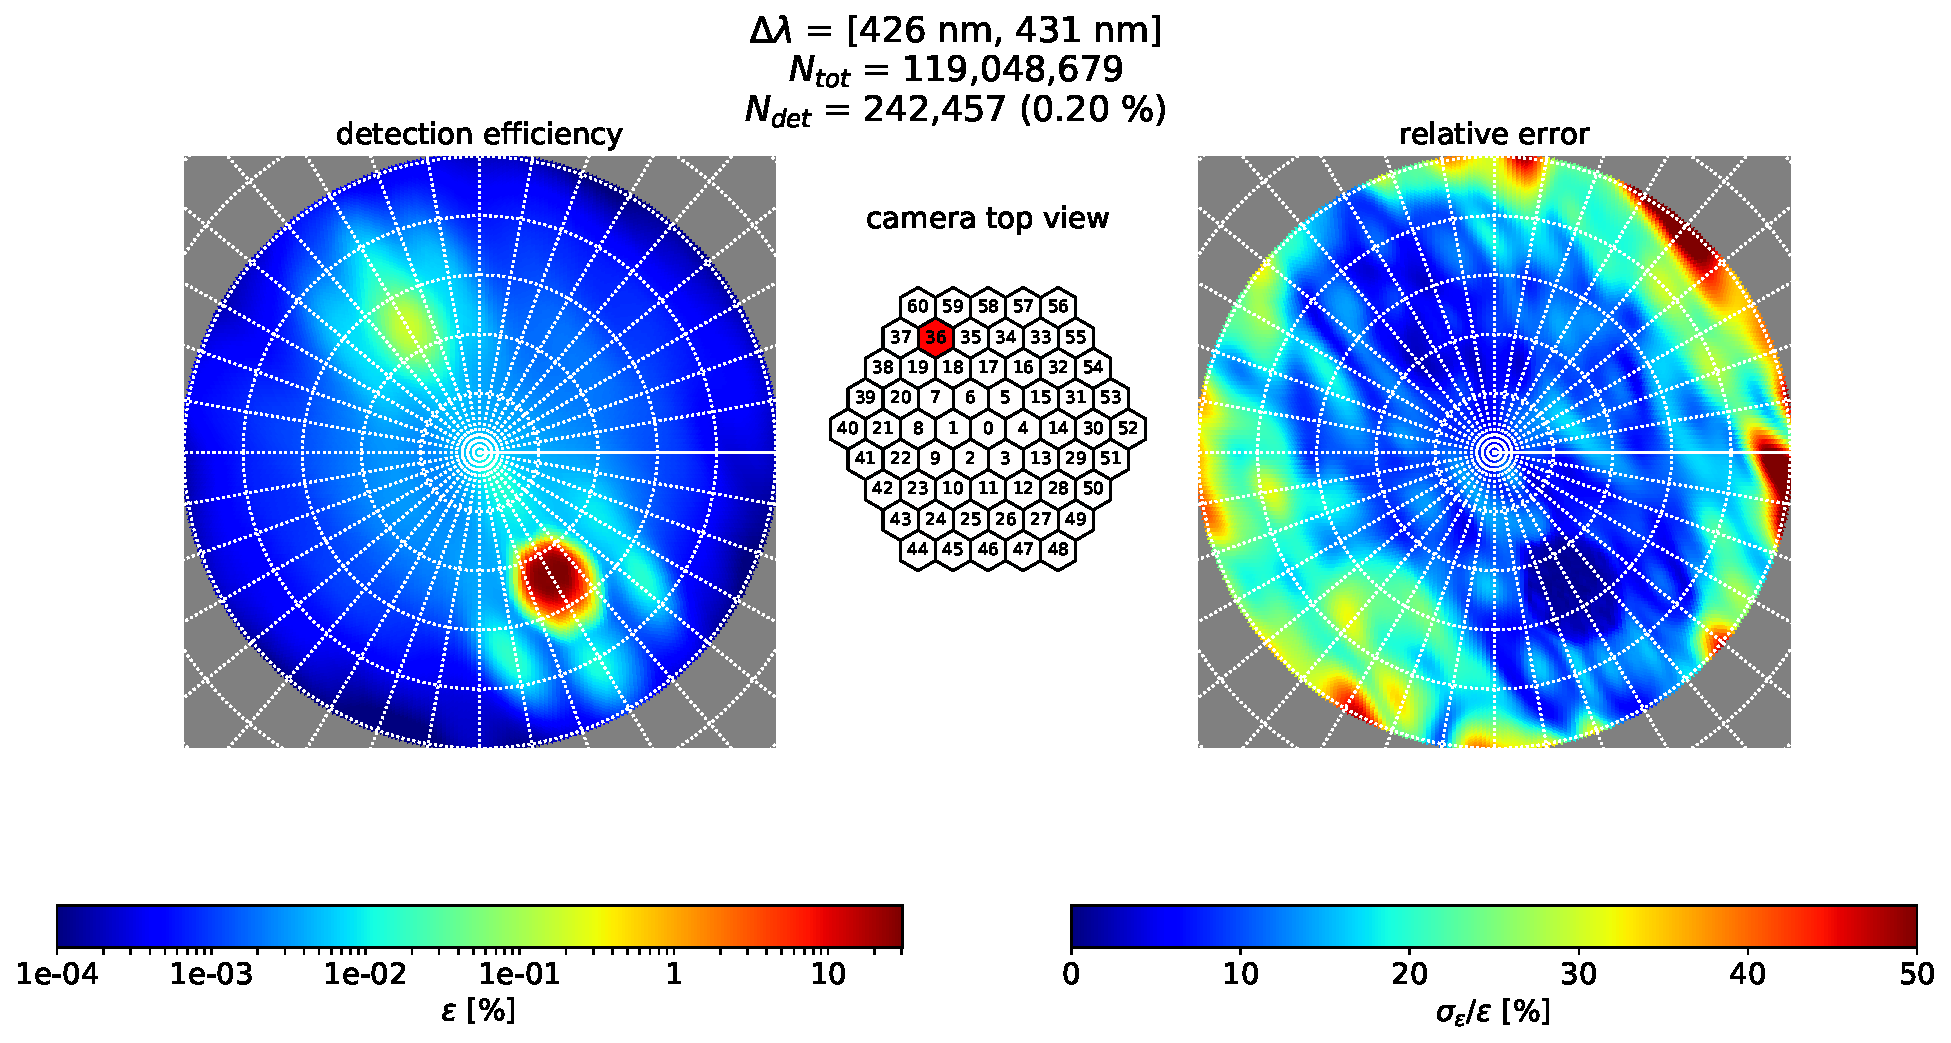
\includegraphics[width=\textwidth]{deteffmaps/deteff_wvl428.5nm_px36_view10.0deg.pdf}
		\subcaption{Pixel 36 on \enquote{quasi-symmetry} axis.}
		\label{deteff:offaxis_px:3}
	\end{subfigure}
	\caption[Detection efficiency maps for some off-axis pixels]{\textbf{Detection efficiency for maps some off-axis pixels.} Similar plots as in figure~\ref{deteff:full_cam} but now for individual camera pixels at the wavelength range with maximum efficiency. Three pixels on symmetry axes are chosen. The two pixels shown in (\subref{deteff:offaxis_px:1}) and (\subref{deteff:offaxis_px:2}) are on real symmetry axes while the third pixel in (\subref{deteff:offaxis_px:3}) is on a symmetry axis of the camera plane but not with respect to the squared SiPMs.}
	\label{deteff:offaxis_px}		
\end{figure}

\section{Lookup Table (LUT)}

As the detection efficiency maps are ready now, one has to think about a way to access the information as fast as possible. Usually, this is done by storing the parameterization function evaluated at certain points in a multidimensional array structure known as \textit{lookup table}. Afterwards, events can be \enquote{diced} with the given information yielding count histograms for the camera -- named \textit{images}.

\subsection{LUT Production}\label{sec:lut_production}

First of all, one has to define how to iterate over the given information. In this case, one starts with a photon direction $(\theta,\phi)$ translated into the corresponding HEALPix number~$HP$ and the wavelength~$\lambda$ of this photon which is assigned to the proper wavelength bin~$\Delta\lambda$. The result then should be the response of each pixel to the very same photon, i.e. how probable is it for the photon to be detected in camera pixel $i$. In order to achieve this, one can evaluate the detection efficiency maps by fist considering just one HEALPix. For this HEALPix, the detection efficiency for all wavelength bins and all camera pixels is read out, which is shown exemplary in figure~\ref{lut:transpose_example}. 

\begin{figure}[H]
	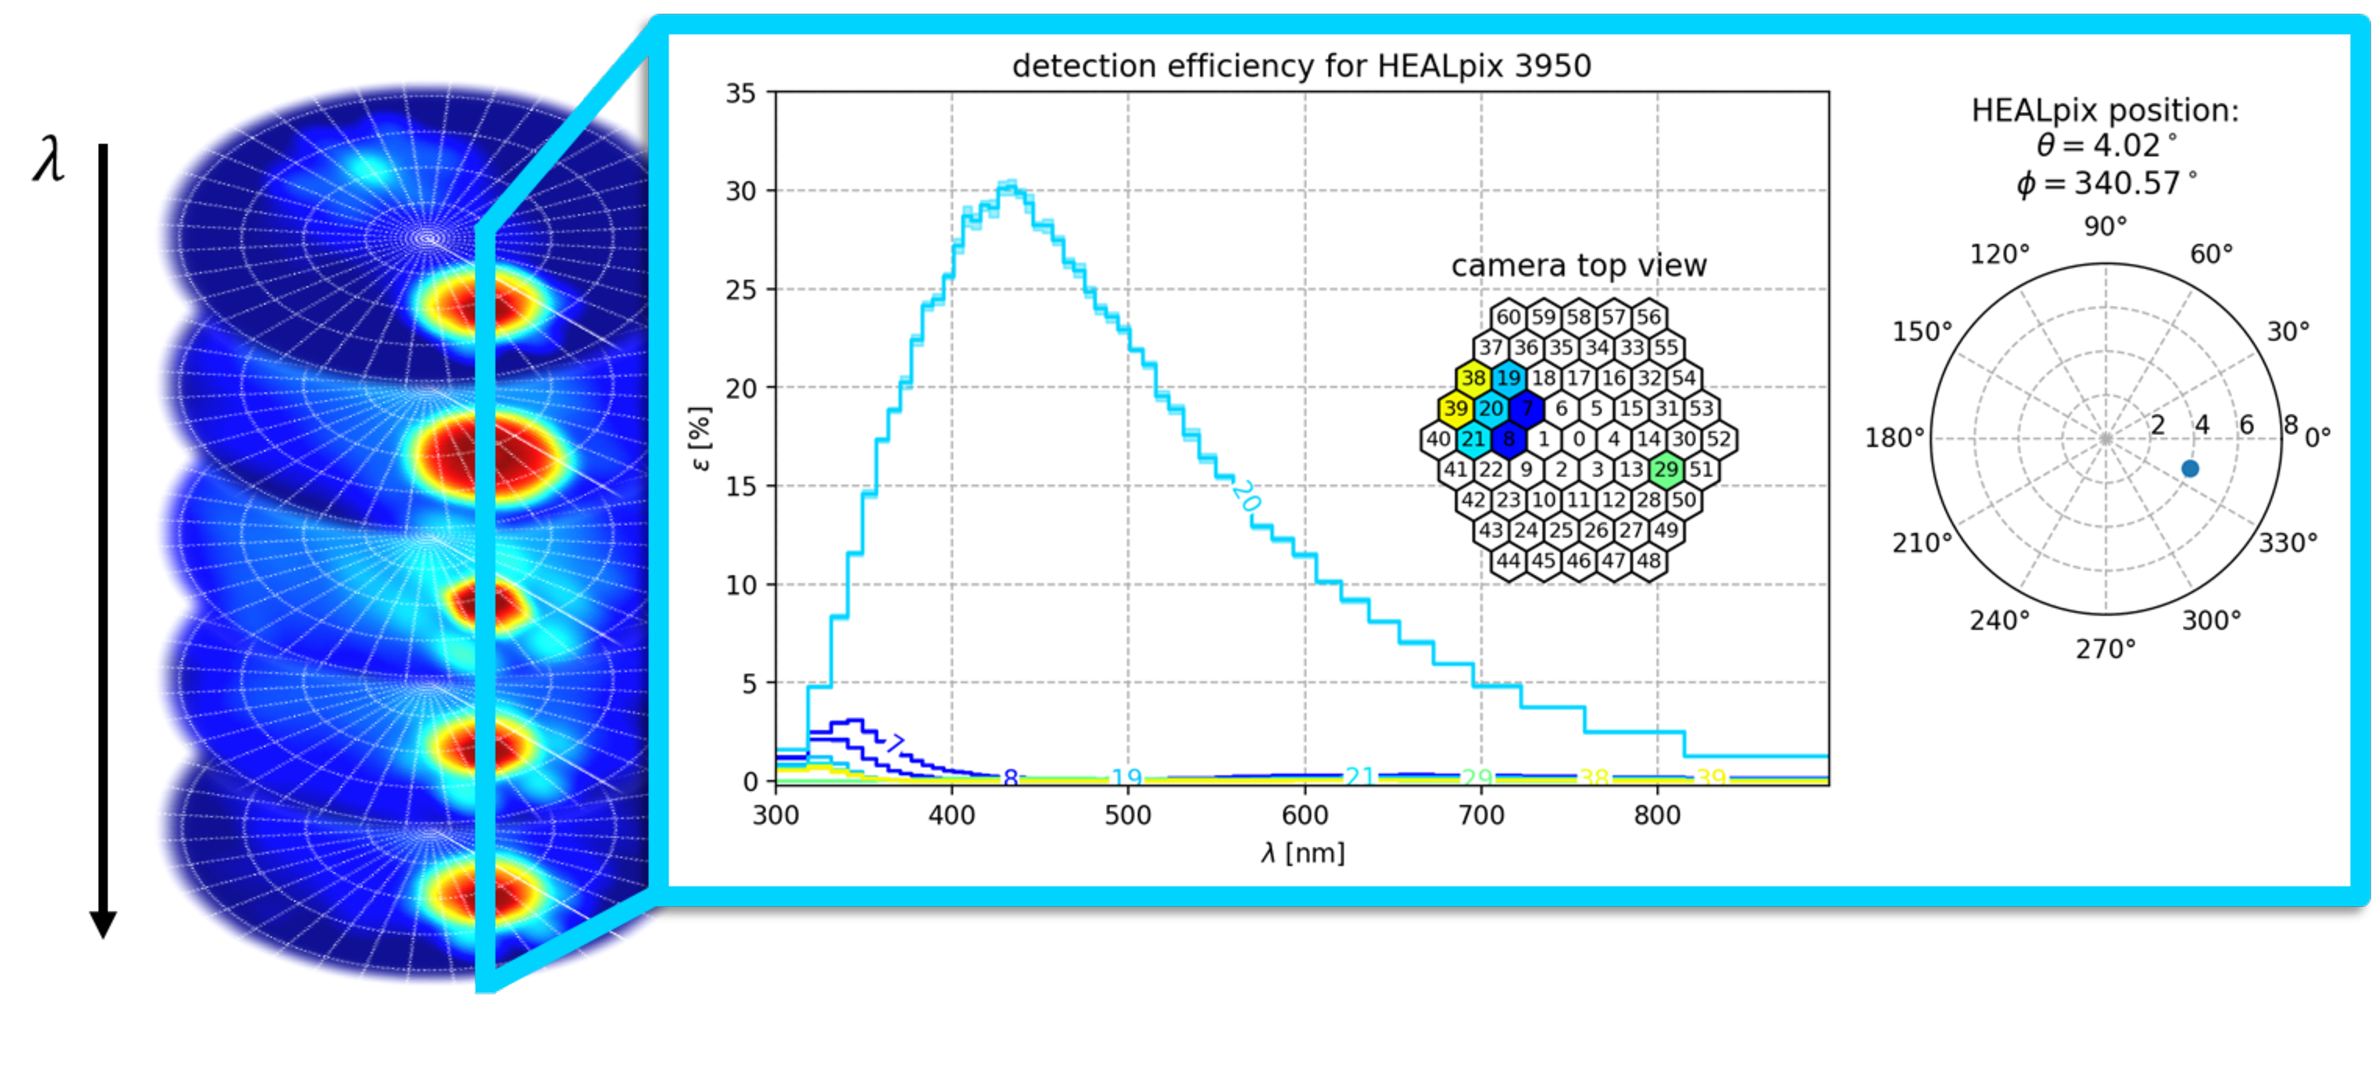
\includegraphics[width=\textwidth]{LUT_transposition_example.pdf}
	\caption[Visualization for the lookup table transposition]{\textbf{Visualization for the lookup table transposition.} A certain HEALPix (here: $HP=\num{4890}$) is considered. For one camera pixel, the detection efficiency is read from the maps throughout all wavelength bins. In this example, some maps for pixel \num{20} are chosen. Doing this for all camera pixels yields to the blue-framed plot. For the considered HEALPix one gets the wavelength-dependent detection efficiency for each camera pixel. The \enquote{camera top view} plot shows the camera as seen from the lens. Pixels that have a maximum detection efficiency greater than~\SI{0.1}{\percent} are emphasized with colors. The detection efficiency functions of all other pixels are not plotted. Besides, the HEALPix center coordinates are given with a polar plot.}
	\label{lut:transpose_example}
\end{figure}

By iterating over each HEALPix of one gets $N_{HP}\times N_{\Delta\lambda}$ pixel-by-pixel detection efficiency arrays where $N_{HP}$ is the total number of HEALPix covered by simulation and $N_{\Delta\lambda}$ the number of wavelength bins. These sub-arrays are further named as $\epsilon_{HP,\Delta\lambda}$ and contain the detection efficiency $\epsilon_i$ for each camera pixel $i$ (also called \textit{pixel response}). 

Additionally, one can even improve the structure of these sub-array by not just saving the single responses $\epsilon_i$ ordered by pixel number, but saving the cumulative responses. Then, the $k$-th of totally \num{60} elements in the sub-array is defined as 
\begin{align}
	\epsilon^\text{abs}_k = \sum_{i=0}^{k} \epsilon_i\,,
	\label{eq:eps_cumulative}
\end{align}
i.e. $\epsilon^\text{abs}_k$ is the probability to detect the photon in any pixel with number $i\in[0,k]$. Additionally, it is
\begin{align}
\epsilon_k^\text{abs} < 1\,,
\end{align}
where the last element $\epsilon_{60}^\text{abs}$ is the total detection probability of the camera and distances between the elements represent the responses of the individual camera pixels. The advantage of saving the cumulative sum rather than actual responses gets clear in the next section~\ref{sec:lut_readout}. Schematically, the lookup process can be described by
\begin{align}
	\gamma \rightarrow
	\begin{cases}
		(\theta,\phi) & \rightarrow HP\\
		\lambda & \rightarrow \Delta\lambda
	\end{cases}
	\Rightarrow \epsilon^\text{abs}_{HP,\Delta\lambda} = \{\epsilon^\text{abs}_k\}_{k=0}^{60}\,.
\end{align}\\

The HEALPix resolution used for parameterization of \iceact is $N_\text{side}=\num{512}$. With $\theta_\text{max}=\SI{10}{\degree}$, this results in a total \enquote{active} HEALPix number of $N_{HP}=\num{24420}$. Additionally, the wavelengths are divided into $N_{\Delta\lambda} = \num{50}$ bins in the interval $[\SI{272}{\nano\meter},\SI{900}{\nano\meter}]$ (cf. section~\ref{sec:wvl_binning}). For the \num{61} pixel camera this results in $N_{HP}\cdot N_{\Delta\lambda}\cdot \num{61} = \num{74481000}$ numbers to be saved. The needed disk space for this lookup table is \SI{284}{\mebi\byte} by using \SI{32}{\bit} float as data type\footnote{Since also the information about wavelength binning, HEALPix model, and maximum simulated zenith angle has to be included, the lookup table file might need slightly more space}.

\subsection{LUT Readout -- \enquote{Event Dicing}}\label{sec:lut_readout}

Now that the data is ready, an evaluation algorithm has to be elaborated. In the following, the principle to evaluate $N$ photons is described step by step.

\begin{enumerate}
	\item For each direction the corresponding HEALPix number is calculated.\footnote{In this thesis, the evaluation algorithm is implemented with Python. For HEALPix calculations, the package \textit{healpy} is used.}
	\begin{align}
		\{(\theta_i, \phi_i)\}_{i=1}^N \rightarrow \{HP_i\}_{i=1}^N
	\end{align}
	\item Only valid photons are evaluated. A photon is valid if its HEALPix number~$HP_i$ is in the lookup table -- i.e. below the cutoff -- and if its wavelength~$\lambda_i$ is in the wavelength range covered by the lookup table $[\lambda_\text{min},\lambda_\text{max}]$. $N^\ast\leq N$ photons are valid. Invalid photons are counted.
	\begin{align}
		\text{valid} \coloneqq HP_i < N_{HP} \wedge \lambda_i \in [\lambda_\text{min},\lambda_\text{max}]
	\end{align} 
	\item For all $N^\ast$ photons, the corresponding wavelength bin is determined.
	\begin{align}
		\{\lambda_{i^\ast}\}_{i^\ast=1}^{N^\ast} \rightarrow \{ \Delta\lambda_{i^\ast} \}_{i^\ast=1}^{N^\ast}
	\end{align}
	Here, the index of the assigned wavelength bin rather than the actual range is important for the lookup table query.
	\item The actual lookup table query is performed. Thus, every valid photon gets its proper pixel response array.
	\begin{align}
		\{HP_{i^\ast}, \Delta\lambda_{i^\ast}\}_{i^\ast=1}^{N^\ast} \rightarrow \{ \epsilon^\text{abs}_{HP_{i^\ast},\Delta\lambda_{i^\ast}}\}_{i^\ast=1}^{N^\ast}
	\end{align}
	\item For each valid photon $i^\ast$, a random number $r_{i^\ast}\in[0,1)$ is diced and sorted into the corresponding response array. Now, the advantage of saving the cumulative rather than the absolute responses (cf. section~\ref{sec:lut_production}) becomes clear. By definition, the cumulative responses are sorted in ascending order\footnote{This is the case if all numbers are non-negative like it is the case for the camera pixel responses. Otherwise, the cumulative sequence may not be sorted.}. As a result, the position $k$ where the random number is sorted in equals the ordinal number of the camera pixel where the photon is detected. If the random number is sorted in at the \num{61}-th position -- i.e. at the end -- this means that the photon is not detected. The cumulative saving enables a lookup process that is only based on comparative operations which are very fast.
	\item The resulting sorting positions $k_{i^\ast}$ can now be histogramized which gives the final image seen by the camera.
\end{enumerate}

\section{Application on CORSIKA Air Shower Events}

With the lookup table, one can finally produce event displays -- or images -- of simulated air showers. A commonly used toolkit for detailed Monte-Carlo simulation of cosmic-ray air showers is \textit{CORSIKA}\footnote{\textbf{CO}smic \textbf{R}ay \textbf{S}imulations for \textbf{KA}scade}~\cite{corsika:website}. It is capable of simulating the direction and energy of Cherenkov photons which emerge from air showers.\\

The plots in figure~\ref{corsika-events} show some images of air showers simulated with CORSIKA. Three different primaries are induced: proton, iron, and photon (gamma). The wavelength or respectively the energy of Cherenkov photons could possibly simulated directly within CORSIKA as stated before. But this results in a large amount of data and a longer simulation time. Therefore, just the direction of some Cherenkov photons, that hit the detector surface in a certain region is stored. For the lookup process, the wavelength of each photon is drawn from the Cherenkov spectrum shown in figure~\ref{airshowers:cherenkovspectrum} by extrapolating wavelengths above \SI{700}{\nano\meter} with a linear function. More details about possible options with CORSIKA and the simulation process can be found in the CORSIKA manual~\cite{corsika:manual}.\\

In order to take into account the effective area of the telescope, only Cherenkov photons that hit a circular area within a diameter of the glass plate $d=\SI{650.3}{\milli\meter}$. This holds for the case of an upright telescope. For a telescope tilted by a zenith angle $\theta^\ast$, the projected effective area is
\begin{align}
A_\text{eff}^\ast = A_\text{eff}\cos{\theta^\ast}\,.
\end{align}\\

However, the events shown in figure~\ref{corsika-events} are evaluation for the simple case of a single, upright telescope.

\begin{figure}[H]
	\centering
	% protons
	\begin{subfigure}[t]{0.49\textwidth}
		\includegraphics[width=\textwidth]{test-events/01/station_09.pdf}
		\subcaption{}
		\label{corsika-events:1}
	\end{subfigure}
	\hfill
	\begin{subfigure}[t]{0.49\textwidth}
		\includegraphics[width=\textwidth]{test-events/08/station_09.pdf}
		\subcaption{}
		\label{corsika-events:2}
	\end{subfigure}
	\vfill
	% iron
	\begin{subfigure}[t]{0.49\textwidth}
		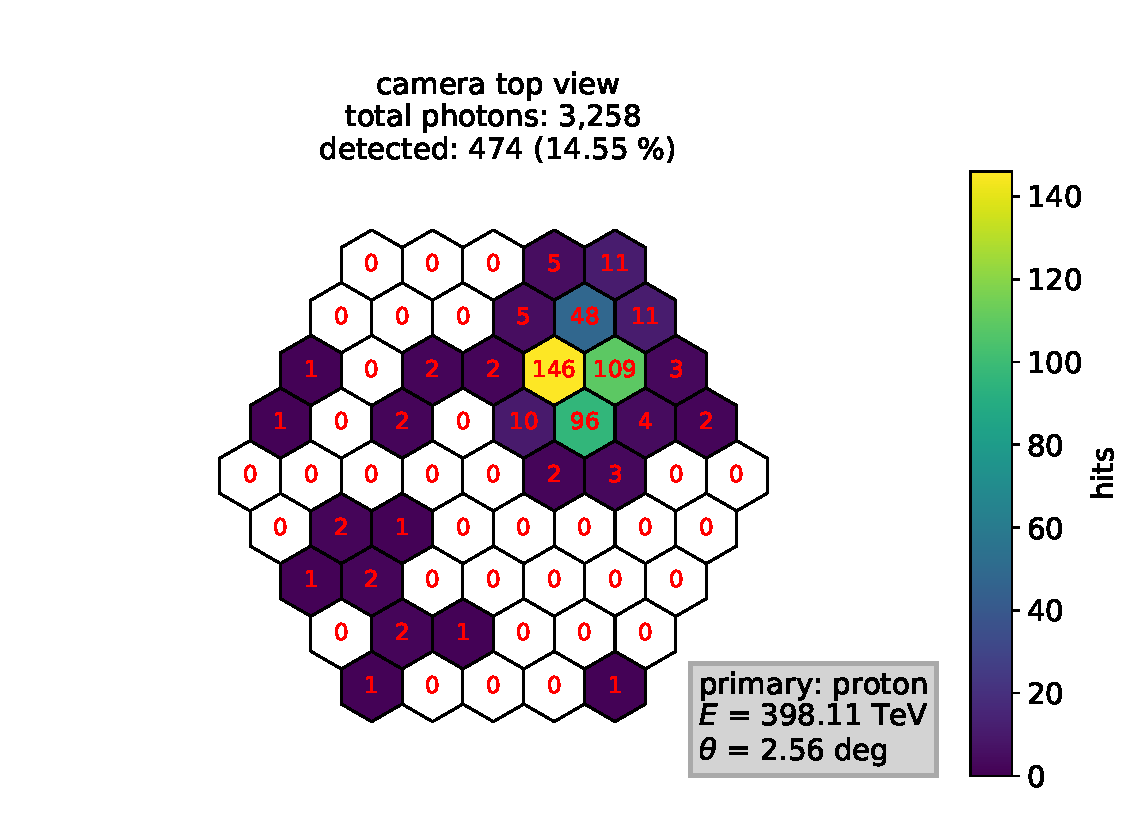
\includegraphics[width=\textwidth]{test-events/07/station_14.pdf}
		\subcaption{}
		\label{corsika-events:3}
	\end{subfigure}
	\hfill
	\begin{subfigure}[t]{0.49\textwidth}
		\includegraphics[width=\textwidth]{test-events/06/station_09.pdf}
		\subcaption{}
		\label{corsika-events:4}
	\end{subfigure}
	\hfill
	% gamma
	\begin{subfigure}[t]{0.49\textwidth}
		\includegraphics[width=\textwidth]{test-events/04/event.pdf}
		\subcaption{}
		\label{corsika-events:5}
	\end{subfigure}
		\hfill
	\begin{subfigure}[t]{0.49\textwidth}
		\includegraphics[width=\textwidth]{test-events/05/event.pdf}
		\subcaption{}
		\label{corsika-events:6}
	\end{subfigure}
	\caption[Camera images diced with lookup table]{\textbf{Camera images diced with lookup table.} The red numbers in the hexagonal pixels count the number of detected photons in the respective pixel. In these events, only the direction of Cherenkov photons is simulated by CORSIKA. The wavelengths of the photons are drawn from the Cherenkov spectrum given in figure~\ref{airshowers:cherenkovspectrum}.}
	\label{corsika-events}
\end{figure}